\documentclass[pdftex,letterpaper,11pt]{article}
\usepackage[font=footnotesize,labelfont=bf]{caption}
\usepackage{amsmath}
\usepackage{booktabs}
\usepackage[inline]{enumitem}
\usepackage[export]{adjustbox}
\usepackage{wrapfig}
\usepackage{subfig}

\usepackage{amssymb,amsfonts} % Add by Xiaofan
\usepackage{amsthm} % Add by Xiaofan
\usepackage{commath} % Add by Xiaofan
\usepackage{algorithmic}
\usepackage{mathtools, nccmath}% Add by Xiaofan
%\usepackage{setspace} % Add by Xiaofan
\usepackage{sectsty} % Add by Xiaofan
\sectionfont{\normalsize}% Add by Xiaofan

\usepackage{array}
% \usepackage[demo]{graphicx}
% \usepackage[title]{appendix}
\usepackage{textcomp}
\usepackage{xcolor}
\usepackage[final]{pdfpages}

% Imported Package

% %\usepackage[USenglish,american]{babel}
% \usepackage{cite}
% \usepackage{amsmath,amssymb,amsfonts}
% \usepackage{algorithmic}
% %\usepackage{graphicx}
% \usepackage{url}
% %\usepackage{array}
% %\usepackage{textcomp}
% \usepackage{xcolor}
% %\usepackage[final]{pdfpages}


\usepackage[compact]{titlesec}
\titlespacing{\section}{0pt}{*0}{*0}
\titlespacing{\subsection}{0pt}{*0}{*0}
\titlespacing{\subsubsection}{0pt}{*0}{*0}

\usepackage[left=1.7cm,top=1.7cm,right=1.7cm,bottom=1.7cm]{geometry}

\usepackage{setspace}
\doublespacing

\graphicspath{{./figures/}}

\let\OLDthebibliography\thebibliography
\renewcommand\thebibliography[1]{
  \OLDthebibliography{#1}
  \setlength{\parskip}{0pt}
  \setlength{\itemsep}{0pt plus 0.3ex}
}

\begin{document}

\theoremstyle{definition}
\newtheorem{theorem}{Theorem}

\theoremstyle{definition}
\newtheorem{definition}{Definition}

\theoremstyle{definition}
\newtheorem{corollary}{Corollary}

\title {\large  \bf \vspace{-10ex}
Theory and Practice (Analysis and Design) Peak Current Mode Control of High-Frequency DC-DC Converters
\vspace{0ex}}
\date{}
\author{Xiaofan~Cui\thanks{X. Cui is with the Department
of Electrical Engineering and Computer Science, University of Michigan, Ann Arbor,
MI, 48109, USA, e-mail: cuixf@umich.edu.}\,,\ \textit{Student Member},~\textit{IEEE},
        and Al-Thaddeus~Avestruz\thanks{A. T. Avestruz (corresponding author) is an assistant professor with the Department
        of Electrical Engineering and Computer Science, University of Michigan, Ann Arbor, MI, 48109, USA, e-mail: avestruz@umich.edu, telephone number: (+1)617-290-4179.}\,,\ \textit{Member},~\textit{IEEE}
        % <-this % stops a space
       % <-this % stops a space
% <-this % stops a space
}
\maketitle
\thispagestyle{empty}
\pagestyle{empty}

\renewcommand{\figurename}{Fig.}


\hspace{-17pt}\textbf{Announcement}: 
This paper has not been presented at a conference or submitted elsewhere previously.\\
\textbf{Abstract}: \\
\textbf{Index Items:}
\newpage
\section{Introduction}\label{sec:Intro}
Although peak (or valley) current mode control (PCC) has been widely used in dc-dc voltage regulator control for a long time, high frequency \footnote{switching frequency $> 1$ MHz} dc-dc converters using PCC are seldomly reported in the literature.

Parasitic ringing is an important bottleneck when implementing PCC for high-frequency dc-dc converters. The severe voltage spikes are common in a high frequency power converts using PCC as shown in \ref{fig:noisecurrent}. In one of our experiments, when these harsh parasitic ringings contaminate current measurements, the inner current loop of a current-mode buck converters using constant on-time (CM-COT) buck converter can actually be unstable. This phenomena challenges the traditional understanding that in CM-COT buck converters, {\color{red} the inner current loop} is deadbeat and stable at all operating points \cite{Redl1981}. In this paper, we provide new theoretical criteria which explain why and predict when this instability phenomena happen.
% We also prove that the stability margin can be improved by slowing down the controller bandwidth.

It is impossible to decrease the parasitic inductance under the level of $n$H under the constraints of the current pc board technology. Therefore, we solve this problem in another way: instead of eliminating parasitic ringings, we show three new compensation techniques which guarantee the PCC to work in harsh parasitic ringing conditions - analog comparator overdrive propagation delay {\color{red}(COPD)}, slope compensation and low-pass filter. We show that the overdrive propagation delay of the analog comparator can be eliminate the effect of parasitic ringing interference on the plant. We explain that the slope compensation, which is widely used in fixed-frequency PCC, can also be used in variable-frequency PCC to reject the parasitic ringing interference. We claim that a low-pass filter with cut-off frequency slower than switching frequency can still result in a good performance.
Furthermore, unlike the traditional compensation design methods based on rule-of-thumbs and design experiences, we show a rigorous analysis tool to help designer with the design procedure.

PCC is advantageous in high-frequency and fast-transient-response dc-dc converters over the other traditional control methods including voltage-mode control and ripple-based control. Peak current mode control shows significantly faster transient response and is much easier to design than the voltage mode control \cite{erikson2007}. Power converter plant in PCC architecture is usually a lower order system compared to voltage mode control because the PCC architecture eliminates the transient from duty cycle to inductor current by measuring and commanding inductor current \cite{Bram2015tpel}. A low order plant makes the compensator design easier and more robust. Peak current mode control is more robust to the output capacitor parasitic and can be applied in any types of dc-dc converters compared to the ripple-based method \cite{Redljian2009tpel}. PCC sense and control the inductor current directly while the ripple-based control has to rely on the assumption that the capacitor voltage contains the information of inductor current. PCC does not rely on the output capacitor and load information, but the ripple-based method can even go in instability if the ESR or ESL is not appropriate. PCC can fix the switching frequency more easily but ripple based control suffers a lot from the jittering in switching frequency. PCC can provide a tight DC voltage regulation. Another important benefit is that PCC naturally does cycle-by-cycle over current protection to the power stage, hence the fault protection design can be simplified. 

Among many PCC architectures in literature, direct PCC using the mixed-signal hardware implementation is one of the most popular approach because it has both fast transient response and programmable flexibility. By whether the inductor current is sensed or not, state-of-the-art PCC can be direct PCC methods and indirect methods. Among direct PCC methods, mixed-signal implementation is the most promising because it shares the benefits of fast transient response and ability to be quickly online tuned to adapt to fast varying operating points. Analog implementation is the most traditional implementation method: The output voltage is processed by an error amplifier and the result is compared with the sensed current signal by an analog comparator \cite{Kaz2006tcs}. Although the design methods are well-established and it is not hard to obtain high control bandwidth, good dynamic performance is not always guaranteed in a wide operating voltage range because {\color{red} electrical dynamics} of circuits change with output voltage operating points and load conditions \cite{erikson2007}. Digital implementation guarantees the programmable flexibility of the adaptive voltage regulation: An analog-to-digital converter (ADC) is added to discretize the sampled inductor current. Then the quantified current is compared with the current command in through digital logic. The implementation of the inductor current sampling can be referred to \cite{Lilee2008APEC}. It is not suitable for high-frequency converter because a high-speed sampler is required. Mixed-signal hardware implementation \cite{Prodic2011tcs} \cite{Huerta2012} combines the advantages of both analog and digital implementations. A common mixed-signal structure includes a digital voltage control loop and an analog current loop.

Because of the difficulties in measuring inductor current in high-frequency power converters, several indirect PCC are proposed. However, currently proposed indirect PCC  still cannot outperform the direct PCC.
Current-programmed control constructs the inductor current waveform using the priori-model and control the inductor current indirectly by duty ratio.
The classic current-programmed control \cite{Chendragan2003} is sensitive to the time-varying uncertainties of the inductor model and the input/output voltage measurement. Although \cite{Taeed2014} improves the method by measuring the actual current at two points every cycle and calculate slope, the prediction error is still inevitable because in some applications where the inductor current can go highly non-linear \cite{Ahsanuzzamanprodic2012apec} \cite{DiCapua2016}. Hence curve fitting using 2 sample points can cause significant errors. Another method in \cite{Chattopadhyay2006} claim a control algorithm which is stable under the incorrect current ramp estimation, but the proposed method cannot guarantee fast transient response.
A V\textsuperscript{2}I\textsubscript{c} method by \cite{Huerta2013} measures and control the capacitor current which contains the inductor current information.
However, a complicated impedance matching network has to be designed to compensate the output capacitor parasitic 
\cite{Huerta2009a}. Several derivative output ripple voltage (DORV) techniques get the capacitor current information by differentiating the capacitor voltage \cite{Mai2008} \cite{Chen2017}. Although the methods avoid the complicated capacitor current measurement, it is vulnerable to noises because of derivative calculation. 
Several papers combine the aforementioned current mode control techniques with other control methods, for example, \cite{Huang2002} combines the peak current mode control and the ripple-based control. \cite{Cheng2014a} is the digital version of \cite{Huang2002}. \cite{Cheng2013} and \cite{Liu2018} combines ripple-based control with the current-programmed control and derivative output ripple voltage technique respectively. There also exist a few current-mode control methods which is not within the aforementioned category, for example, \cite{Kurokawa2016} uses the inductor current feed-forward in voltage mode control. \cite{Saggini2004} Implements a current-programmed control with an synchronously sampled output voltage.

Main factors which restrict the control bandwidth of dc-dc converters using PCC are low-loss switching devices, high-speed digital control devices and low circuit parasitics. Recently, the commercial GaN FET already has low enough switching losses which enables the high frequency DC-DC converter using hard switching \cite{Huang2014c}.
People can get access to high speed digital control device. For example, a commercial ADC with precision over 10 bits can have sampling latency lower than 50\,ns \cite{dsAD9215,dsMAX1214}, In the market, there are several types of DAC with settling time lower than 20\,ns \cite{dsLTC1666, dsAD9744} and FPGA with main clock higher than 400\,MHz \cite{dsARTIX72018}. 

Circuit parasitic is more important in implementing direct PCC because the parasitic ringing causes the current measurement and current command error. However, the frequency and time constant of ringing are limited by the minimal parasitic inductance on PCB technology which is in the level of nH. The induced voltage spike is comparable to the voltage on the measurement resistor. Among a few existing works which tackles the high frequency PCC converters problem, either the power level or the power efficiency is sacrificed. Some paper decrease the power rating to avoid ringing interference, but this limited the application area. \cite{Huerta2012} shows a 5MHz converter on board with output power lower than 5\,W. Some use integrated circuit to eliminate the parasitic, but this limit the power level of the circuit. \cite{Trescases2011} reports a 3MHz PCC buck converter on IC. Another method is introducing extra power losses to improve the signal to noise ratio. For example, using damper or snubber to attenuate the energy as well as the amplitude of the ringing. Increasing the sensing resistor value to get a much cleaner current ramp. However, considering the conduction loss is proportional to the square root of current $P_{\text{loss}} = I^2R$ but the signal-to-noise ratio is proportional to the current $V = IR$, this method does more harm than good in large output current applications like voltage regulator modules(VRMs). 

In this paper, instead of trying to eliminate the parasitic ringing, we use several compensation techniques to stabilize the PCC high-frequency power converters even in harsh parasitic ringing conditions. We first exhibit a novel model on the mechanism of how ringing influences the power converter plant and control. Based on the model, we show the rigorous analysis tool to study stability and performance of practical DC-DC converter using PCC. Several compensation techniques are compared and discussed under the analysis tools.

\begin{figure}
\begin{minipage}{0.32\textwidth}
    \centering
    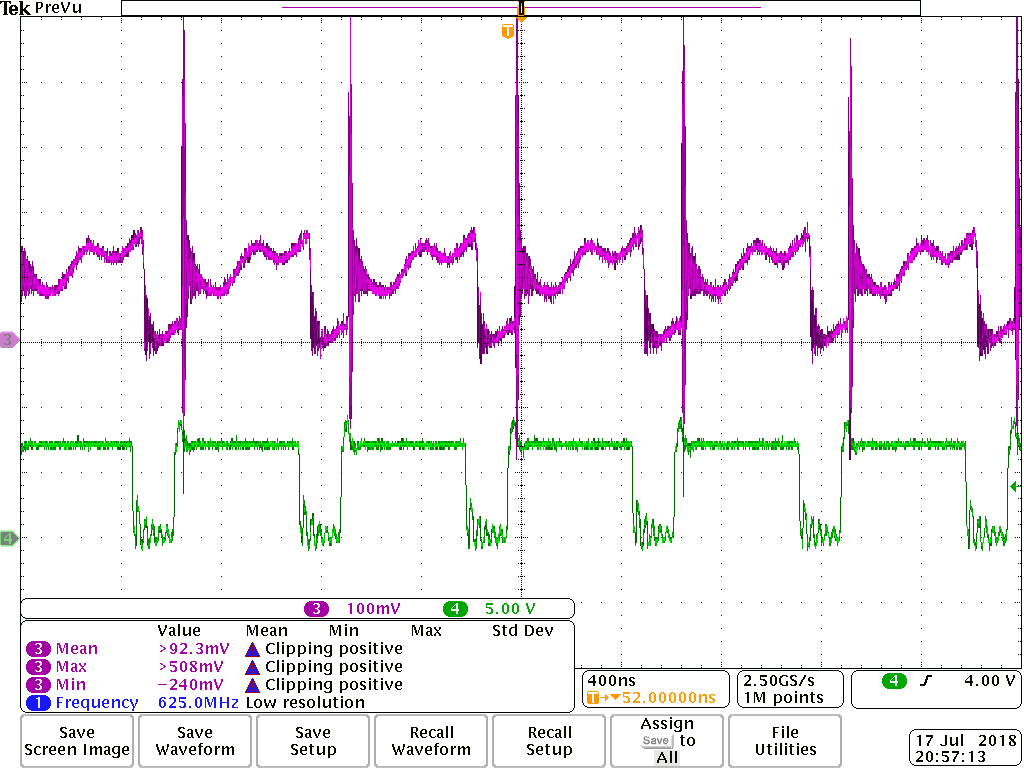
\includegraphics[width=\textwidth]{Figure/section1/ripplecurrent.png}
    \caption{ \label{fig:noisecurrent} Measured inductor current of a digitally-controlled CM-COT boost converter.}
\end{minipage}
%~
% \begin{minipage}{0.32\textwidth}
%     \centering
%     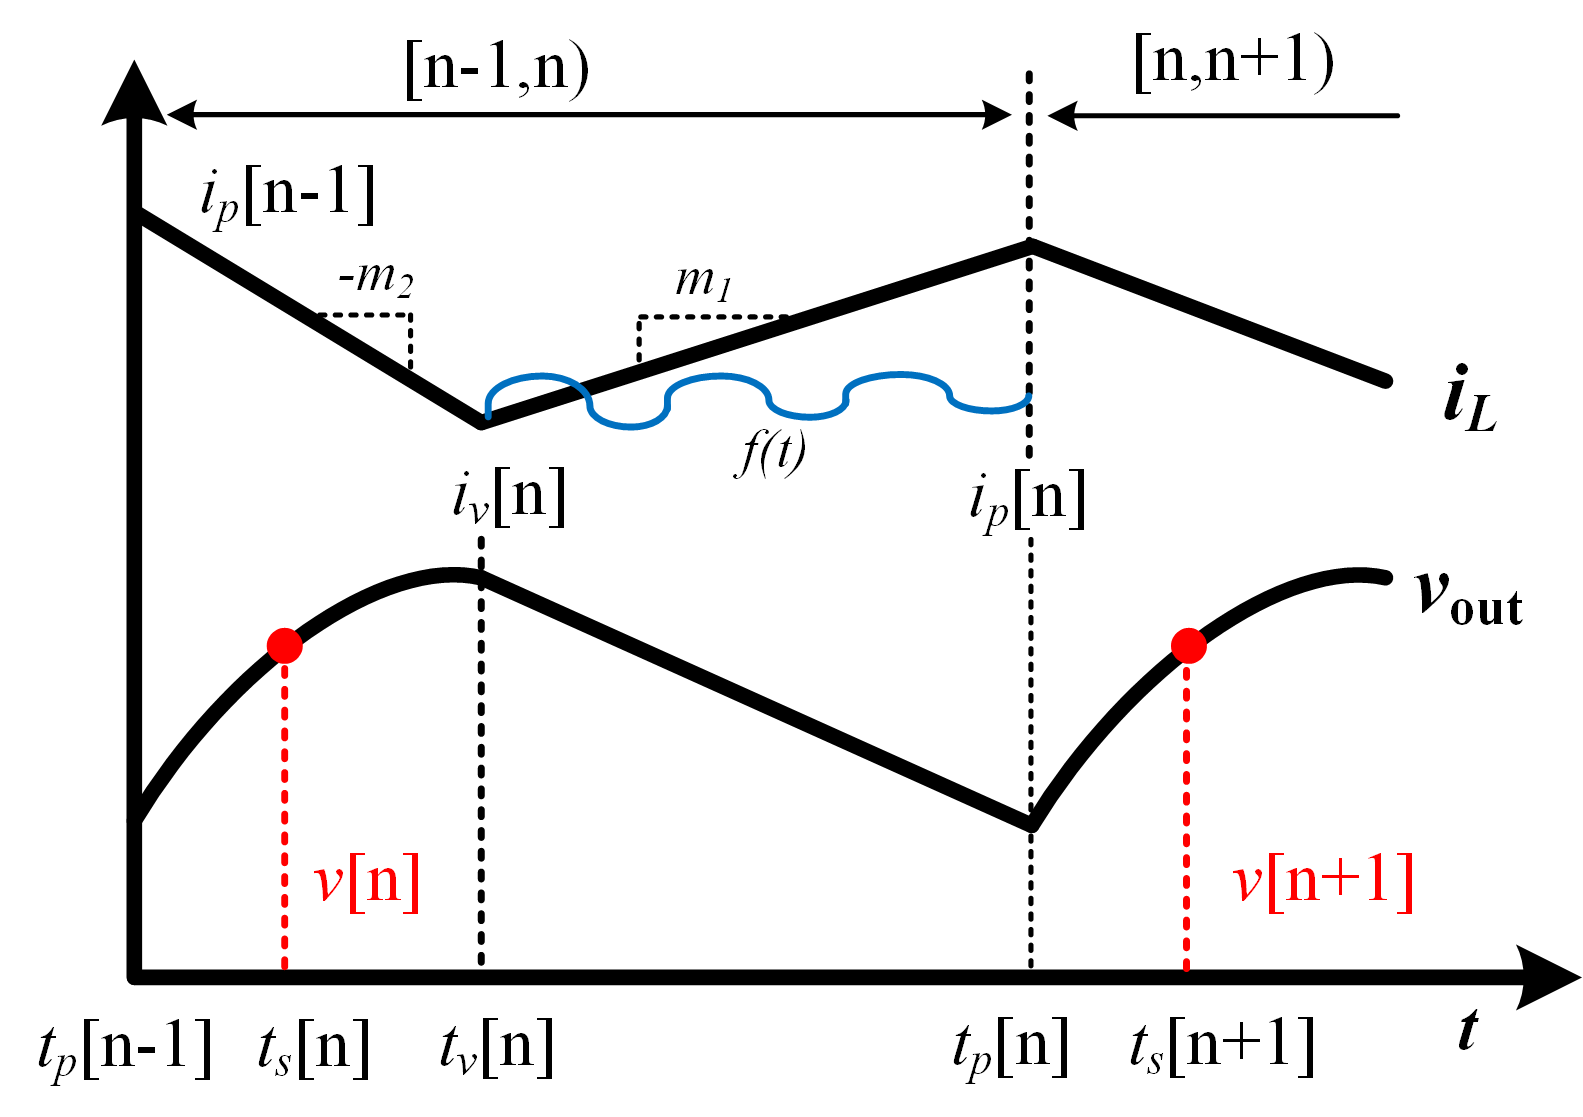
\includegraphics[width=\textwidth]{Figure/section2/eboostwaveform.png}
%   \caption{\label{fig:lcwavefrom} Inductor current and capacitor voltage waveforms of a digitally-controlled CM-COT boost converter.}
% \end{minipage}
~
% \begin{minipage}{0.32\textwidth}
%     \centering
%     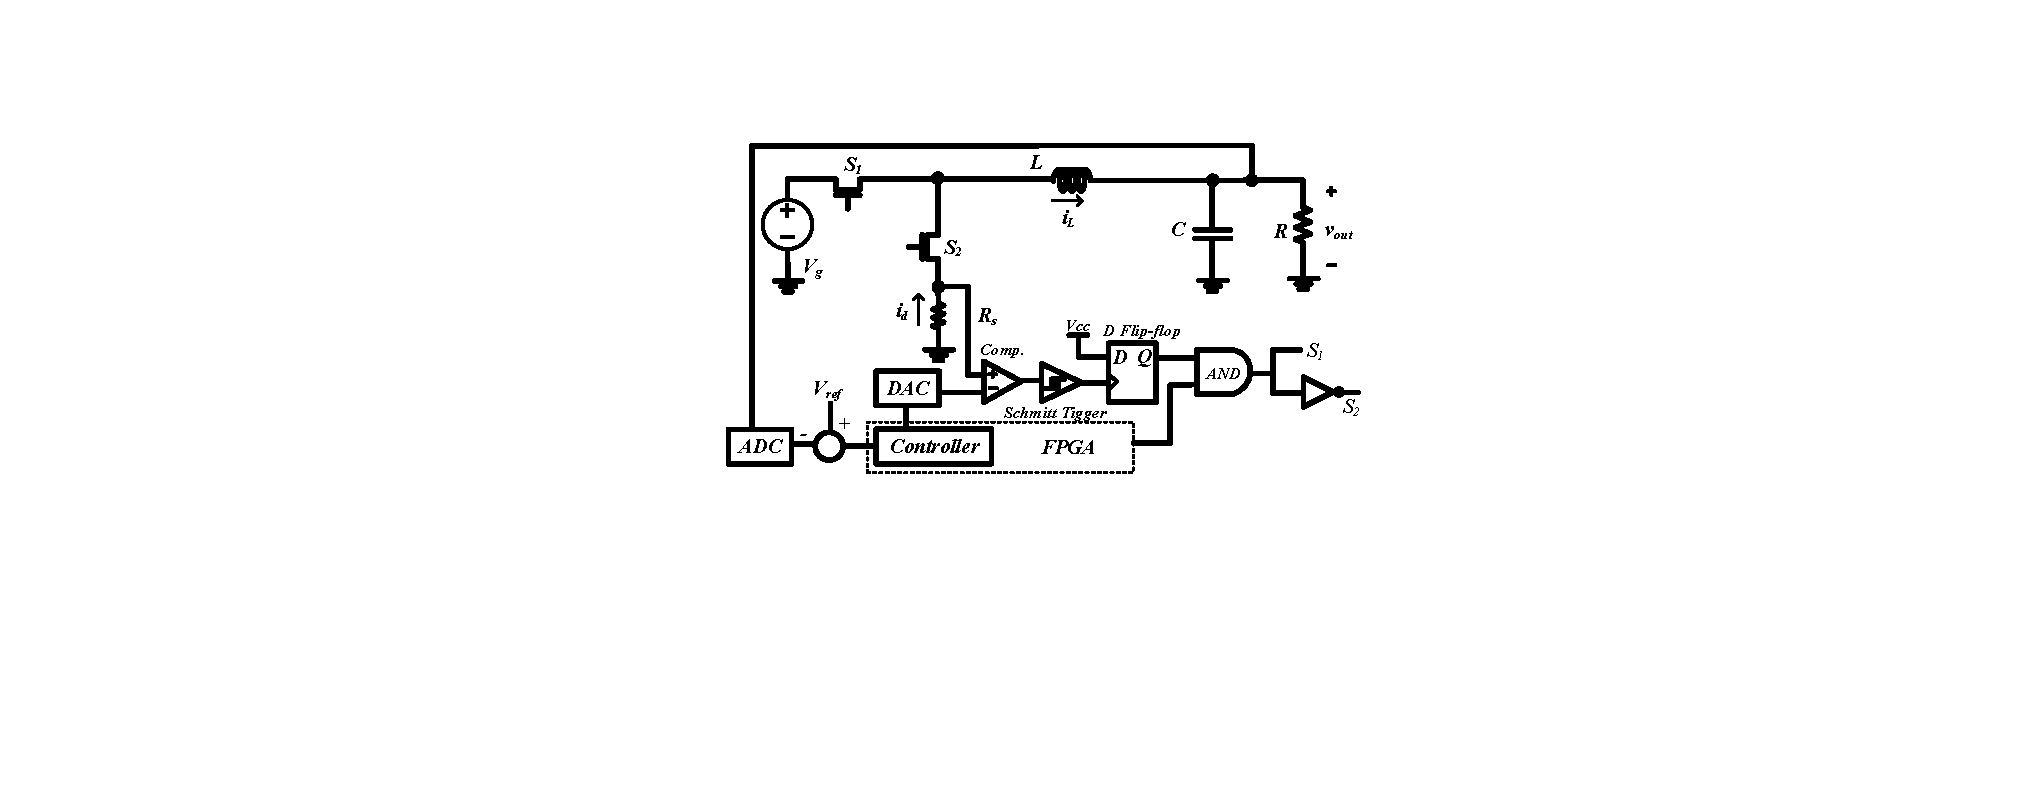
\includegraphics[width=\textwidth]{Figure/section2/currentdetection.pdf}
%     \caption{\label{fig:currentdection} Analog valley-current controller for constant-on-time
%     current-mode buck.}
% \end{minipage}
\end{figure}


\section{Modeling} \label{sec:modeling}

% \begin{figure}
% \begin{minipage}{0.45\textwidth}
% \centering
% \subfloat[\label{fig:classD_rect_sch1} A licking tiger ]{\includegraphics[width=0.7\textwidth]{tiger1.jpg}}\\
% \subfloat[\label{fig:classD_rect_sch2} A mother tiger]{\includegraphics[width=0.7\textwidth]{tiger2.jpg}}
%   \caption{ \label{fig:classD_rect_sch}Adorable tigers}
%   \vspace{-10pt}
% \end{minipage}
% \qquad
% \begin{minipage}{0.45\textwidth}
%     \centering
%     \includegraphics[width=\textwidth]{tiger3.jpg}
%      \caption{ \label{fig:classD_rect_analysis}A smiling tiger}
%      \vspace{-10pt}
% \end{minipage}
% %\vspace{-10pt}
% \end{figure}

The traditional assumption of piece-wise linear inductor current is invalid in practical high-frequency dc-dc converters. Instead, it is more accurate to model the measured inductor current as a ramp added by an interference function.
We illustrate a new model of interfered inner current loop. We found that the reasons of long-time settling and instability in the practical converter can be effectively explained by this model. We first define the interference function as following: 
\begin{definition}
$f(t)$, the interference function in continuous time satisfies the following properties \begin{enumerate*} [label=(\roman*)]  \item $f(t)$ is cycle-invariant; \item $f(t)$ has a bounded amplitude of $[0, A_{\text{max}}]$ and a bounded frequency spectrum of $[\omega_{\text{min}}, \omega_{\text{max}}]$.
\end{enumerate*} 
\end{definition}

\begin{figure}
\begin{minipage}{0.32\textwidth}
    \centering
    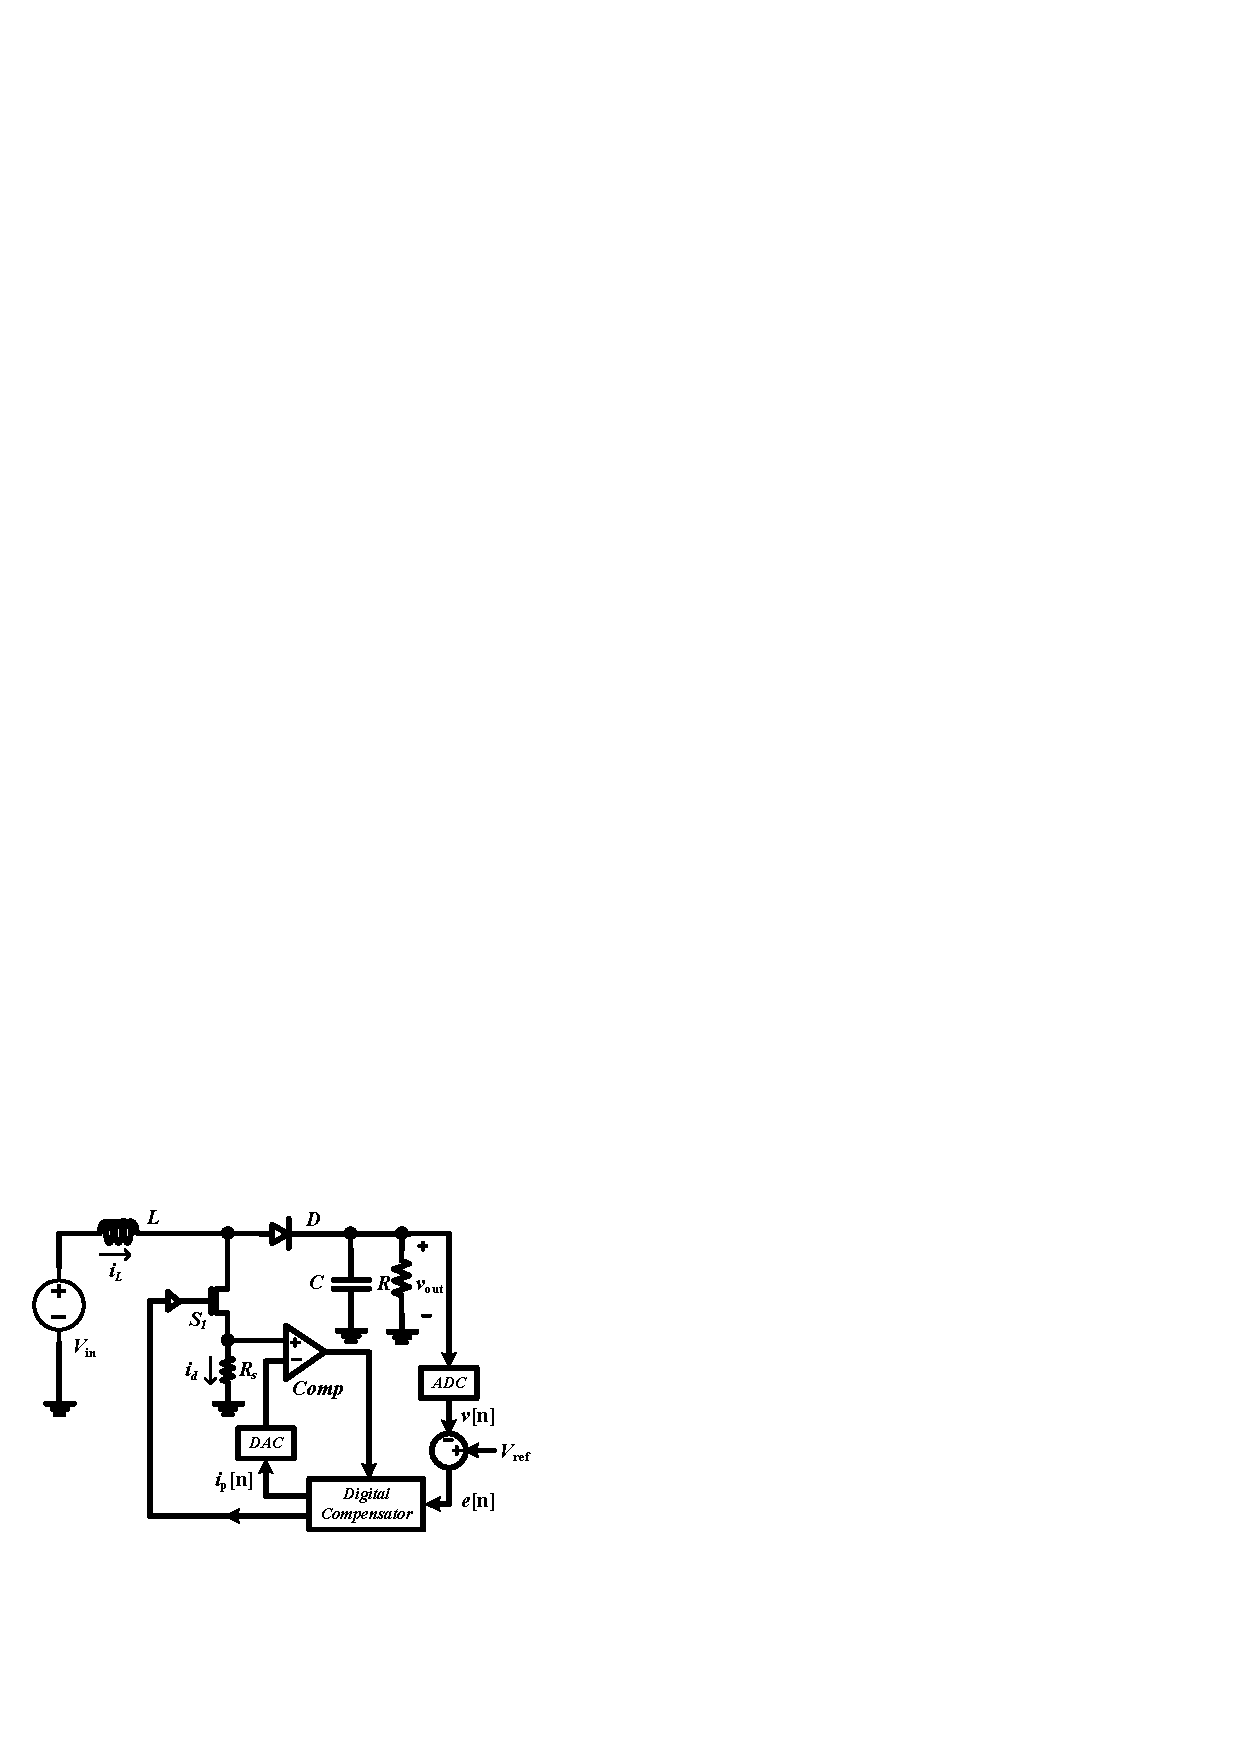
\includegraphics[width=\textwidth]{Figure/section2/schematiceboost.pdf}
    \caption{ \label{fig:eboostschmatic} Schematic diagram of a digitally-controlled CM-COT boost converter.}
\end{minipage}
~
\begin{minipage}{0.32\textwidth}
    \centering
    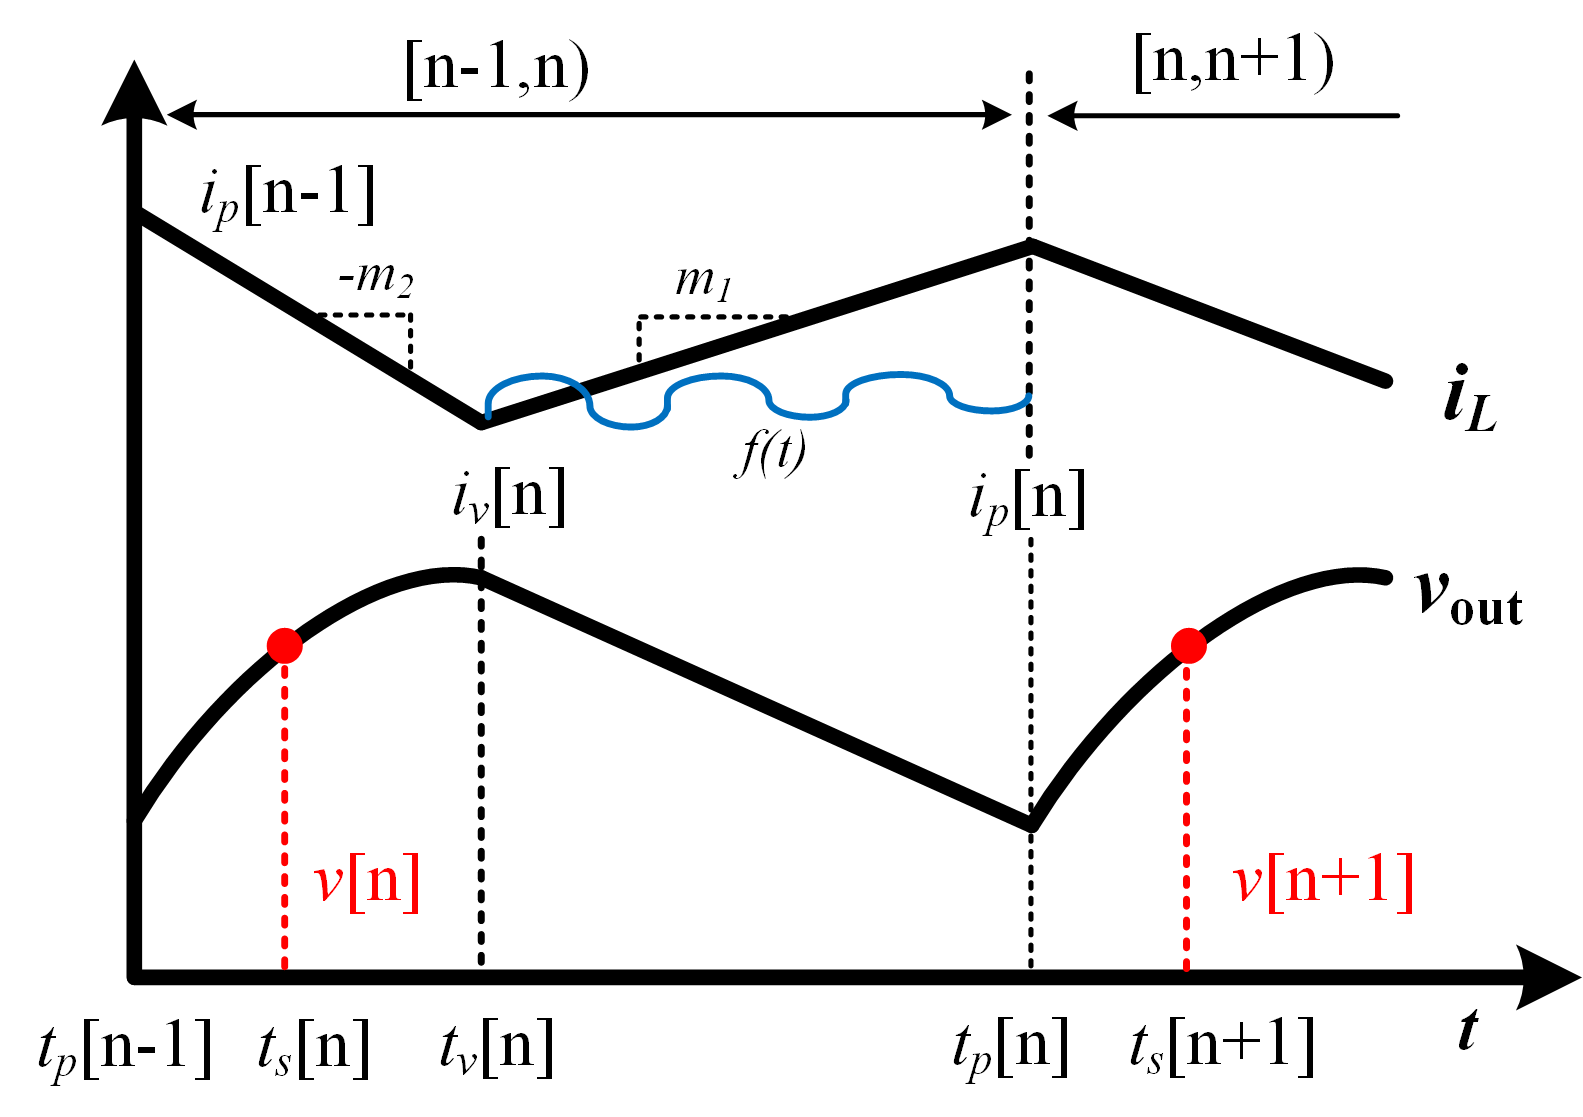
\includegraphics[width=\textwidth]{Figure/section2/eboostwaveform.png}
  \caption{\label{fig:lcwavefrom} Inductor current and capacitor voltage waveforms of a digitally-controlled CM-COT boost converter.}
\end{minipage}
~
\begin{minipage}{0.32\textwidth}
    \centering
    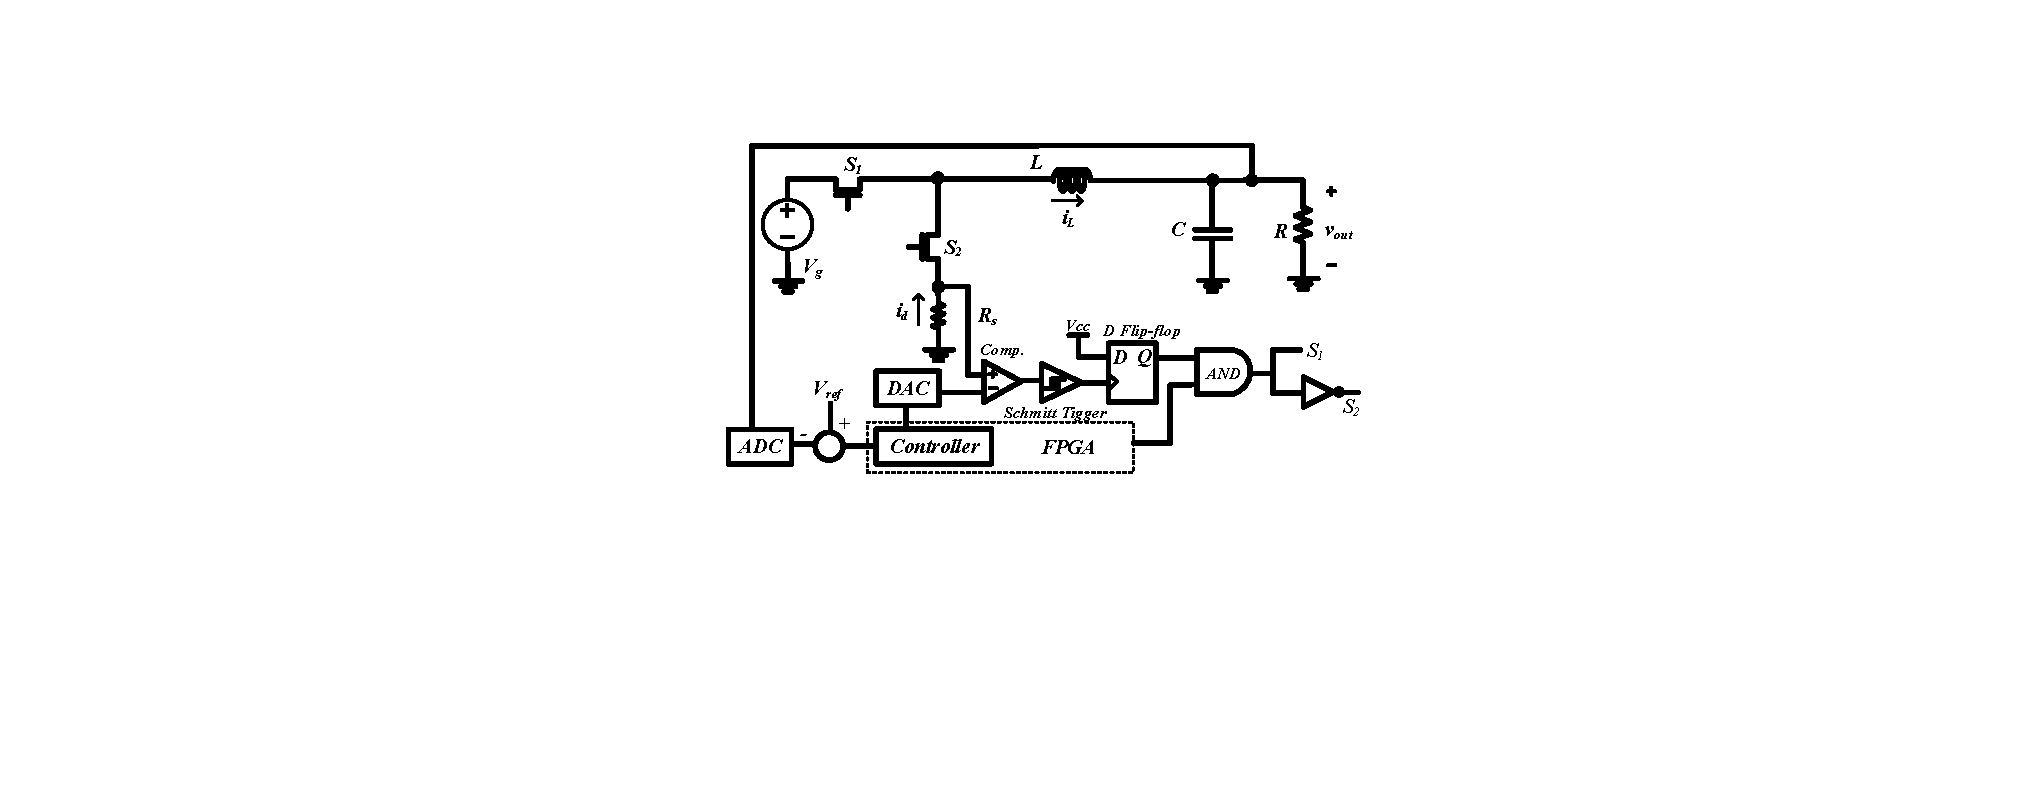
\includegraphics[width=\textwidth]{Figure/section2/currentdetection.pdf}
    \caption{\label{fig:currentdection} Analog valley-current controller for constant-on-time
    current-mode buck.}
\end{minipage}
\end{figure}

The example converter plant we used is a current-mode boost converters using constant off-time (CM-COT boost converter) as shown in Fig.\;\ref{fig:eboostschmatic}.
$i_c[n]$ is the current command from the outer loop every cycle. Our model of the interfered inner current loop can by described by following difference equations:
\begin{align} \label{sys:innerloop}
i_p[n] &= i_p[n-1] - m_2t_{\text{off}} +m_1t_{\text{on}}[n], \\
i_c [n] &= i_p[n] +f(t_{\text{on}}[n]).
\end{align}
The $I_e$ and $T_{\text{on}}$ at equilibrium can be obtained by letting $i_p[n+1] = i_p[n]$, $t_{\text{on}}[n+1] = t_{\text{on}}[n]$. $I_e$ and $I_c$’s relationship are govern by an implicit function $g(I_e, I_c) = 0$. We define an explicit mapping $\mathcal{T}: \mathcal{R}_+ \rightarrow \mathcal{R}_+$ from the inductor current command $I_c$ to the actual inductor current $I_e$ in steady state.

Although no assumptions mathematically guarantees that mapping $\mathcal{T}$ is a single-valued and monotonically non-decreasing explicit function. However, our special design using first-event-triggering mechanism guarantees these properties.
As shown in Fig\;\ref{fig:multieventtrigger}, the possibile triggering time instants can be $t_1$, $t_2$,$t_3$ or $t_4$. The D flip-flop in Fig\;\ref{fig:currentdection} always latch the first comparator detection, which is then reset by the FPGA at the next switching cycle. This design guarantee $t_1$ to be the triggering time instant. A generic function $\mathcal{T}$ is like the shape in Fig\;\ref{fig:functionT}. 
One defect of the function $\mathcal{T}$ is that it might includes jump discontinuity points. For $I_e \in [I_{f_1}-I_{f_2}]$ or $I_{f_3}-I_{f_4}$, there is no correct peak current command $I_c$ which can position the real pwak current.
\begin{definition}
we define the \emph{unreachable equilibrium set} $U\!E \triangleq [I_{f_1},I_{f_2}] \cup [I_{f_3},I_{f_4}],\ldots$. Lebesgue measure of the $U\!E$ is $\lambda(U\!E)$.
\end{definition}
We do not recommend having $\lambda(U\!E) \neq 0$ for control practice because the inner current loop will not be able to position the current to wherever the outer loop controller wants. We give the following theorem without proof to show the relationship between $\lambda(U\!E)$ and interference function $f(t)$.
\begin{theorem} \label{th:equexcond}
$\mathcal{T}$ is an onto-function if and only if the measured inductor current waveform $m_1t+f(t)$ is strictly monotonic.
\end{theorem}
\subsection{Stability}
Under the condition of Theorem \ref{th:equexcond}, we would like to study the stability of the equilibrium. Suppose the equilibrium is at $i_p[n] = I_e$, $t_{\text{on}}[n]= T_{\text{on}}$, $i_c[n] = I_c$, 
We translate the equilibrium to the origin by defining $\tilde i_p[n] = i_{p}[n] - I_{e}$, $ \tilde t_{\text{on}}[n] = t_{\text{on}}[n] -  T_{\text{on}}, \tilde i_c[n] = i_c[n] - I_c$. 
\begin{align}  \label{ID1}
\tilde i_p[n] &= \tilde i_p[n-1] +  m_1 \tilde t_{\text{on}}[n] \\
\tilde i_c [n] &= \tilde i_p[n] +f(t_{\text{on}}[n]) - f(T_{\text{on}}).
\end{align}
We assume the peak current command $ i_c[n]$ from outer voltage loop is fixed at $I_{c}$. 
% We also assume that the the interference function $f$ is strictly monotonic and odd within the domain of our interests, so that the $f^{-1}$ exists and is an odd function as well,
% \begin{align}
% \tilde i_p[n] &= \tilde i_p[n-1] - m_1 (-\tilde t_{\text{on}}[n]), \\
% - \tilde  t_{\text{on}}[n]  &= f^{-1} (\tilde  i_p[n] - f(T_{on})).
% \end{align}

The resulting system can be formulated into a Lure system as shown in Fig\;\ref{fig:luresystem}. By applying the circle criterion, we prove the following theorem to show the stability conditions for the system (\ref{sys:innerloop}) under any disturbance:
\begin{theorem} \label{th:gloasystab}
The $A_{\text{max}} \omega_{\text{max}} < (m_1/2) $ if and only if the inner current loop is \emph{globally asymptotically stable}.
\end{theorem}
\begin{proof}

\end{proof}

\subsection{Performance}
In system (\ref{sys:innerloop}), we view the current command sequence $\tilde i_c [n]$ as the input and the peak inductor current sequence $\tilde i_p [n]$ as the output. Ideally, the peak inductor current is assumed to follow the peak-current command with small overshoot and fast speed. However, with interference amplitude increasing, one could expect the convergence speed gradually slow down and overshoot gradually increases. 
 
We show a $Z$-transform method to systematically analyze the performance of system (\ref{sys:innerloop}) including settling time, overshoot and stability margin. 

We linearize the system (\ref{sys:innerloop}) and have
\begin{align} \label{sys:linear}
    \tilde i_p[n] &= \tilde i_p[n-1] +  m_1 \tilde t_{\text{on}}[n], \\
    \tilde i_c [n]  & = \tilde i_p[n-1] + (f^{'}(T_{\text{on}}) + m_1)\tilde t_{\text{on}} [n].
\end{align}
 We define an equivalent local slope $s_0 = f^{'}(T_{\text{on}}) + m_1$, slope ratio $\beta = m_1/s_0$, and pole of inner current loop $a = 1-\beta$. Then system (\ref{sys:innerloop}) can be simplified as 
\begin{align}
\tilde i_p[n] &=  \beta \tilde i_c [n] + a \tilde i_p[n-1].
\end{align}
Note that although the discretized data does not have a uniform corresponding to physical time domain, $Z$-transform can still be applied \cite{Cui2018a},
\begin{align}
    C_2(z) = \frac{\beta}{1- a z^{-1}}.
\end{align}
Ideally, $\beta = 1$, $a = 0$ and the pole of $C_2(z)$ locates at 0, meaning $C_2(z)$ is deadbeat. 
The larger the $|a|$ is, the longer transient under reference step the inner loop will have.

Because of the uncertainty of the derivative of f, While the operating points is moving, the pole $a$ is within the range
%  $ [1 - m_1/(m_1 + m_s + f^{'}_{\text{min}}), 1-m_1/(m_1 + m_s + f^{'}_{\text{max}})]$. 
\begin{align}
a_{\text{min}} &= 1 - \frac{m_1}{(m_1 + m_s + f^{'}_{\text{min}})} \le a \le   a_{\text{max}} = 1 - \frac{m_1}{(m_1 + m_s + f^{'}_{\text{max}})}.
\end{align}

By denoting $a \in [a_{\text{min}}, a_{\text{max}}]$, 
we can analyze the Worst case settling cycles $-log^{-1}(a)$ and Worst case overshoot (ref) and stability margin $\text{max} \{1+a_{\text{min}}, 1-a_{\text{max}}\}$.

Although the performance analysis is in the discrete time ($5S$), the settling time and overshoot in time domain is predictable by settling cycle and overshoot by theorem 2 and 3 \cite{Cui2018a}.


\begin{figure}
\begin{minipage}{0.32\textwidth}
    \centering
    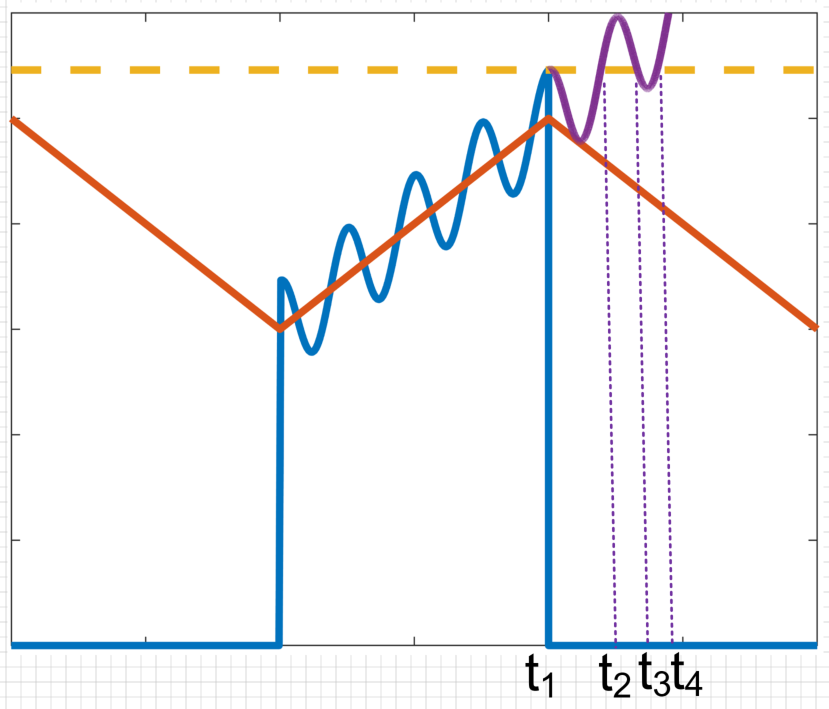
\includegraphics[width=\textwidth]{Figure/section2/Multievent_trigger.png}
    \caption{ \label{fig:multieventtrigger} First-event trigger using D flip-flop.}
\end{minipage}
~
\begin{minipage}{0.32\textwidth}
    \centering
    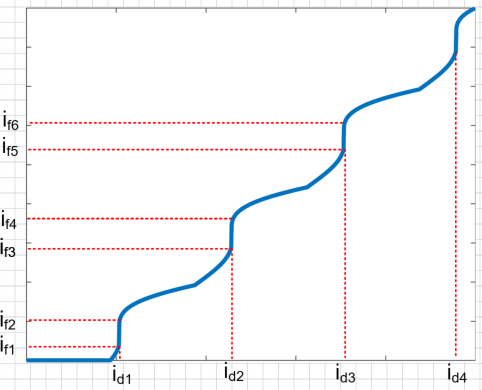
\includegraphics[width=\textwidth]{Figure/section2/functionT.png}
  \caption{  \label{fig:functionT} A common graph for the function $T$.}
\end{minipage}
~
\begin{minipage}{0.32\textwidth}
    \centering
    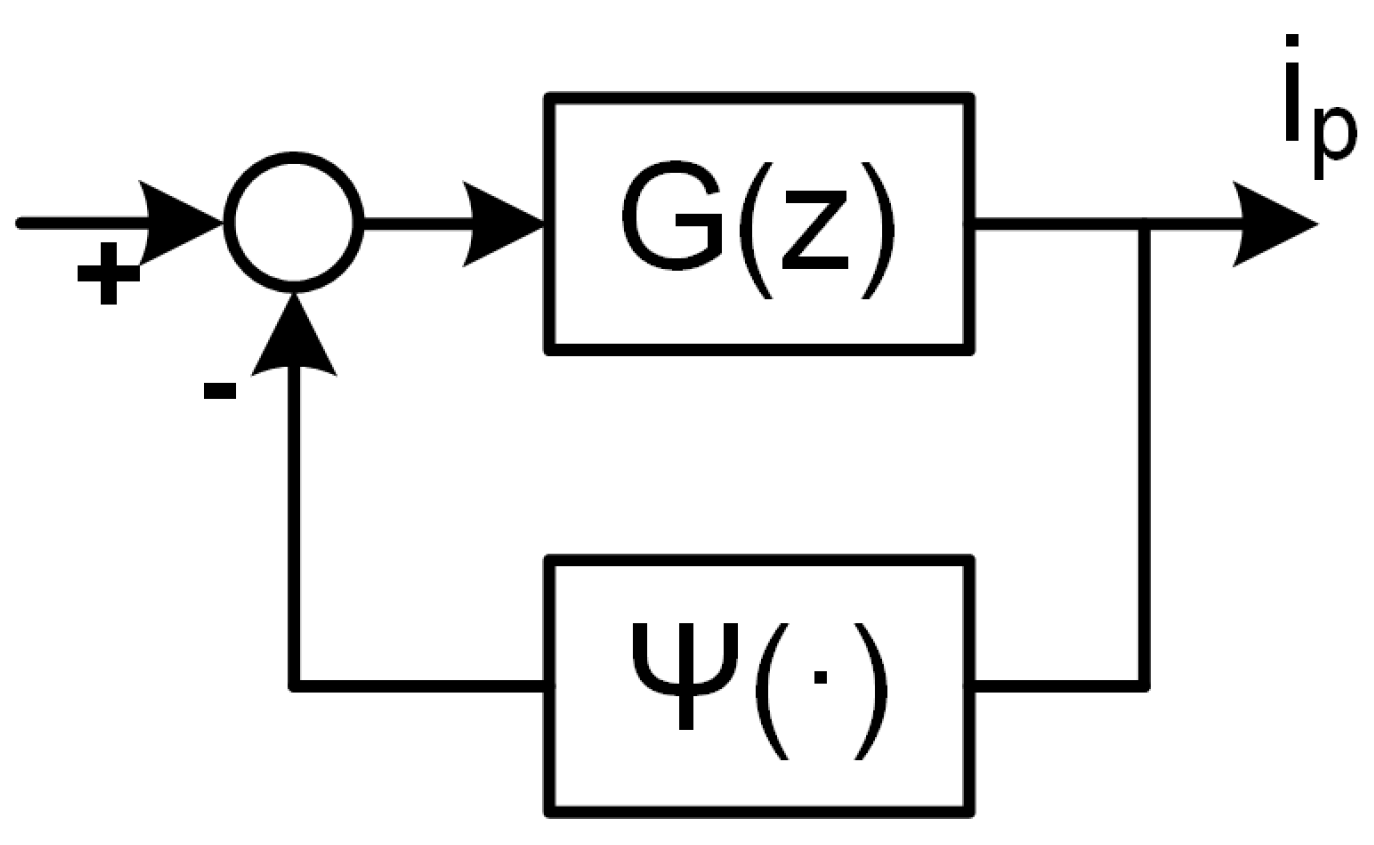
\includegraphics[width=\textwidth]{Figure/section2/luresystem.PNG}
    \caption{\label{fig:luresystem} Lure system representation of the inner current loop.}
\end{minipage}
\end{figure}


A geometric explanation of the current command block dynamics by assuming the noise is a slow varying signal and can be considered as a ramp error


The stability criterion of the current-mode buck converter using constant on-time and current-mode boost converter using constant on-time is given as follows:


\begin{figure}
\begin{minipage}{0.32\textwidth}
    \centering
    \includegraphics[width=\textwidth]{Figure/catsatind3.pdf}
    \caption{ \label{catonsatind} First-event trigger using D flip-flop.}
\end{minipage}
~
\begin{minipage}{0.32\textwidth}
    \centering
    \includegraphics[width=\textwidth]{Figure/ebuckschematicrenew.pdf}
  \caption{  \label{circuitdiagram} A common graph for the function $T$.}
\end{minipage}
~
\begin{minipage}{0.32\textwidth}
    \centering
    \includegraphics[width=\textwidth]{Figure/waveform2.pdf}
    \caption{\label{eboostderivation} Inductor current and capacitor voltage waveforms of a CM-COT buck converter with saturaing inductor.}
\end{minipage}
\end{figure}



% \begin{figure}
% \begin{minipage}{0.49\textwidth}
% \subfloat[\label{fig:licking_tiger}A licking tiger]{\includegraphics[width=0.45\textwidth]{figures/tiger1.jpg}} \quad
% \subfloat[\label{fig:mother_tiger}A mother tiger]{\includegraphics[width=0.45\textwidth]{figures/tiger2.jpg}}
% \caption{\label{fig:beautiful_tiger}Beautiful tigers}
% \end{minipage}
% %%\hfill
% \begin{minipage}{0.49\textwidth}
% \subfloat[\label{fig:smiling_tiger}A smiling tiger]{\includegraphics[width=0.45\textwidth]{figures/tiger3.jpg}} \quad
% \subfloat[\label{fig:phd_tiger}A Ph.D. tiger]{\includegraphics[width=0.45\textwidth]{figures/tiger4.jpg}}
% \caption{ \label{fig:more_beautiful_tiger}More beautiful tigers. Everyone loves tigers.}
% \end{minipage}
% \end{figure}



% \begin{wrapfigure}{r}{0.33\textwidth}
%   \vspace{-20pt}
%   \begin{center}
%     \includegraphics[width=0.32\textwidth]{tiger3.jpg}
%   \caption{ \label{fig:Zrect_eq_model}A smiling tiger}
%   \end{center}
%   \vspace{-20pt}
% \end{wrapfigure}

\section{Solutions} \label{sec:solution}

under harsh ringing when the aformentioned equilibrium existence and stability condition does not hold, we show three compensation techniques which stablize the converter and optimize the performance.

\subsection{Analog Comparator Overdrive Propagation Delay}

A new comparator model considering the overdrive propagation delay
The real comparator has a delay from the input edge to output edge (TI Comp Delay). The delay time is actually variable with respect to the input overdrive, which is called overdrive-propagation delay as shown in Fig\;\ref{fig:copd1} and \ref{fig:copd2}. In high-frequency power converter application, it is not accurate enough to just mode the comparator as an ideal comparator. To take the variable delay into consideration, we show the following variable delay comparator model: We start with the physical model of a comparator is in Fig\;\ref{fig:physicalmodel}. It contains a differential input stage and a multi-stage common-source amplifier output. The load, which is usually the next stage CMOS logic integrated circuit, can be simplified as a capacitor. 
\begin{figure}
\begin{minipage}{0.32\textwidth}
    \centering
    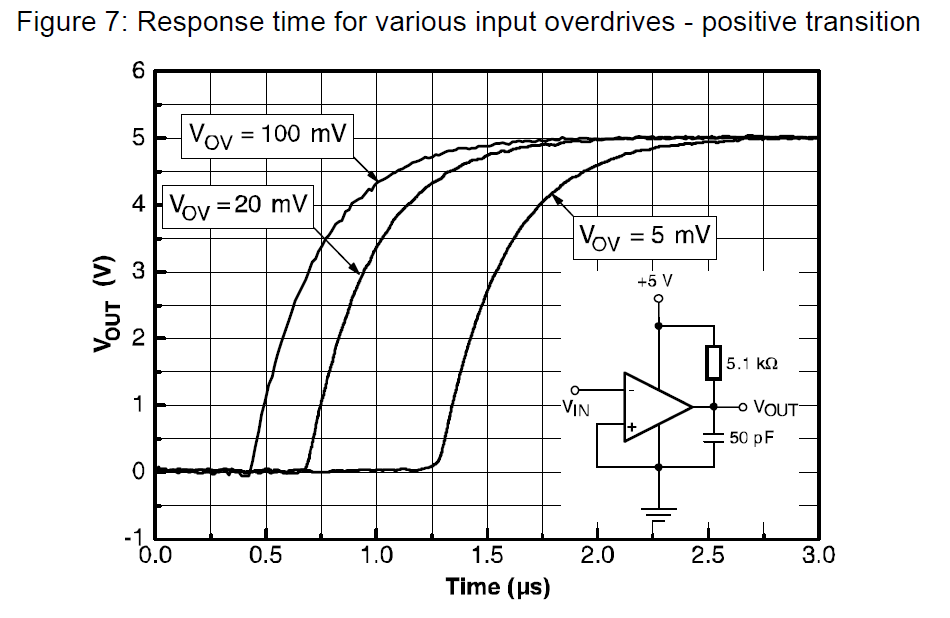
\includegraphics[width=\textwidth]{Figure/section3/copd/copd1.png}
    \caption{ \label{fig:copd1} Comparator Response time various input overdrives.}
\end{minipage}
~
\begin{minipage}{0.32\textwidth}
    \centering
    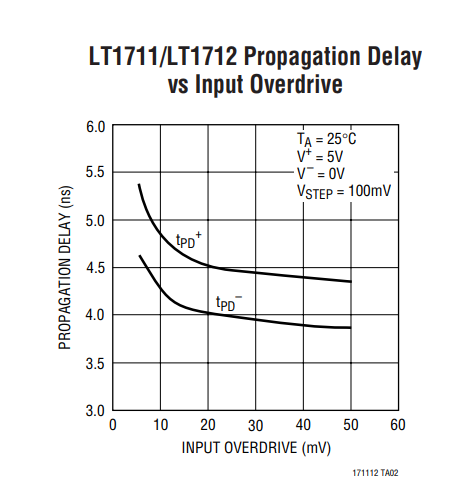
\includegraphics[width=\textwidth]{Figure/section3/copd/copd2.png}
  \caption{  \label{fig:copd2} Comparator Response time various input overdrives(2).}
\end{minipage}
~
\begin{minipage}{0.32\textwidth}
    \centering
    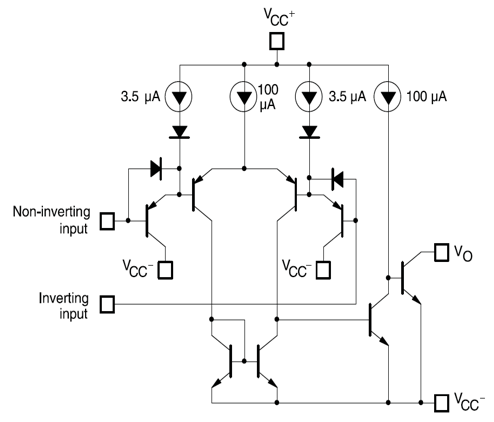
\includegraphics[width=\textwidth]{Figure/section3/copd/physicalmodelcomp.PNG}
    \caption{\label{fig:physicalmodel} Simplified physical model of a comparator.}
\end{minipage}
\end{figure}
To trade-off the balance of model accuracy and analysis complexity, we do reasonable simplification on the comparators system in .Although the large signal gain of the input differential pair is the tanh function of the input overdrive voltage, we use a linear equivalent gain k to approximate the relationship, namely $I_{\text{out}} = k(V_{+} - V_{-})$. We use an integrator block to model the process that output current charges the capacitive load. Then the $V_{\text{th}}$ and an ideal comparator is used to model the process that the following stage is triggered after its input voltage is over the 0.5\,V threshold. 

The simplified model, which we named ''integrator-threshold`` model, proves to capture the main dynamics of the non-ideal comparators by our simulation comparison with the real variable overdrive propagation delay from (LM 193 DS). Fig.3 is the propagation delay from comparator LT1711 datasheet. 
Fig.4 Simulated Overdrive-propagation delay plot using parameters $k = , V_{\text{th}}$. It looks in the similar shape as the simulation result using the following parameters.


The overdrive propagation delay smooths the current command to actual current function $\mathcal{T}$ and improves the stability of the inner current loop.

\begin{figure}
\begin{minipage}{0.32\textwidth}
    \centering
    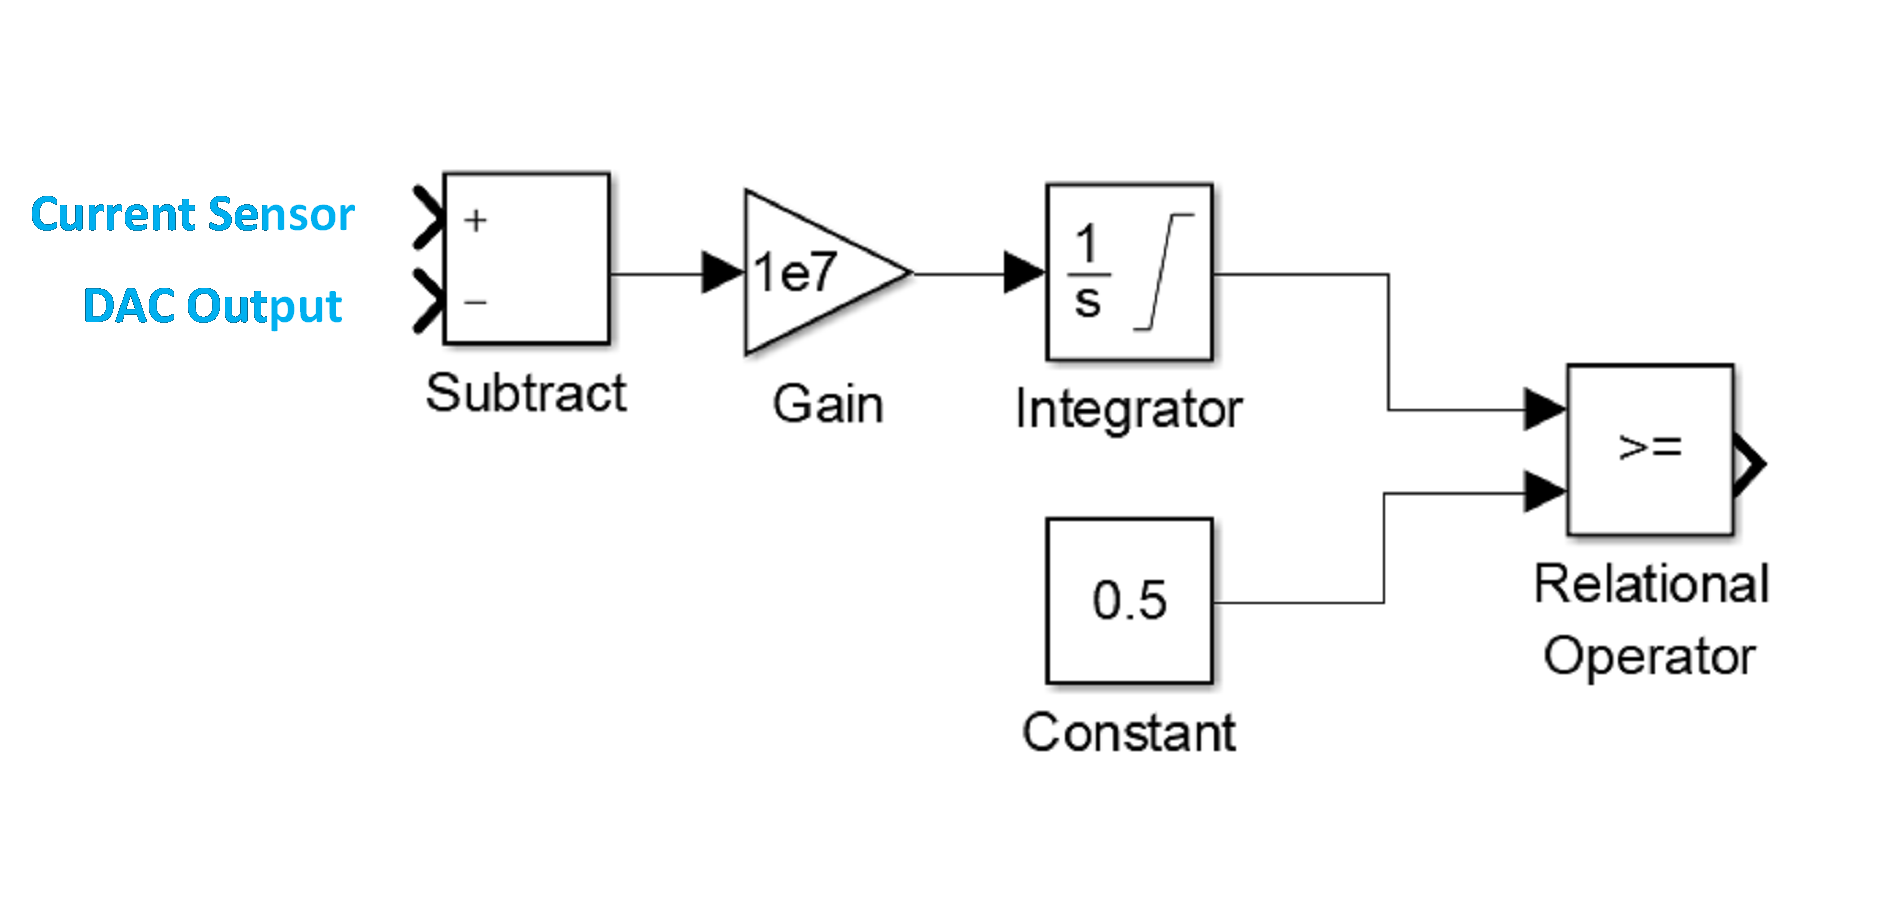
\includegraphics[width=\textwidth]{Figure/section3/copd/mathmodelcomp}
    \caption{ \label{fig:copd1}Simplified mathematic model of a comparator.png}
\end{minipage}
~
\begin{minipage}{0.32\textwidth}
    \centering
    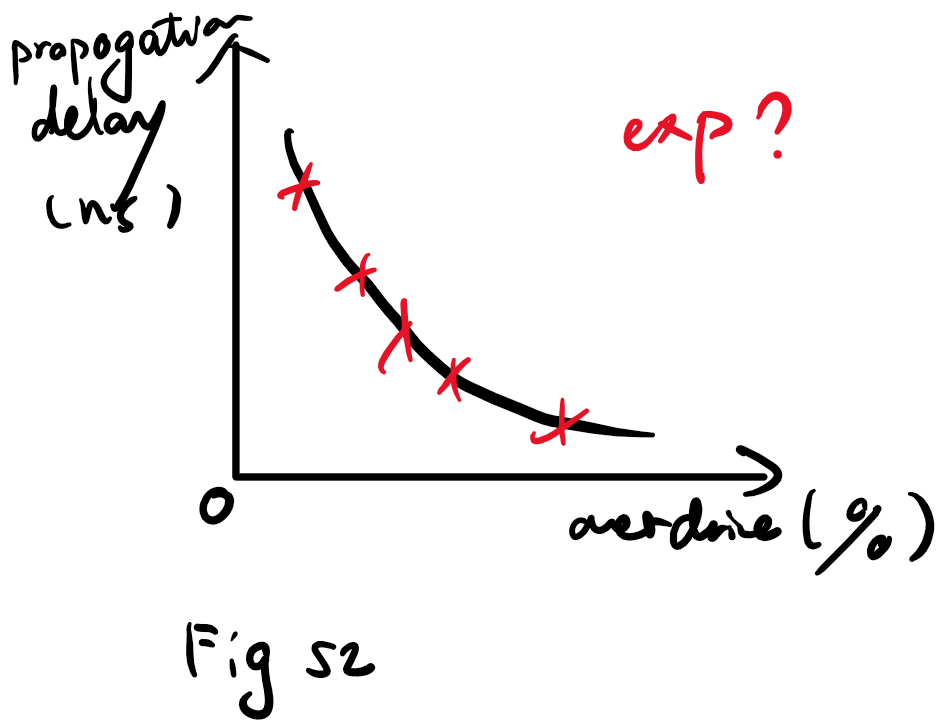
\includegraphics[width=\textwidth]{Figure/section3/copd/simumodelcomp}
  \caption{\label{fig:copd2}Simulated propagation delay using the simplified model of a comparator.}
\end{minipage}
\end{figure}

Fig compares the function $\mathcal{T}$ with and without the overdrive propagation delay. The error gain is a good representative of the overdrive propagation delay. We note that with the increase of the error gain, $\lambda(U\!E)$ decreases. We define the minimum error gain $G_{\text{min}}$ as the error gain which makes $U\!E$ be a zero measurable set. For all $G > G_{\text{min}}$, T is an onto mapping. The algorithm to find out the $G_{\text{min}}$, the minimum gain which make the equilibrium existence condition hold can be found in appendix.

The integrator and threshold mechanism follows
\begin{align} \label{IT}
\int_{t_c}^{t_{\text{on}}} \left(i_p[n-1] - m_2t_{\text{off}} + m_1 t + f(t) - i_c [n] \right) dt = k.
\end{align}
where $k \triangleq V_{\text{th}}/G$ and the crossing time $t_c[n]$ is defined as the solution of equation
\begin{align} \label{DTC}
 m_1 x + f(x)  = i_c [n] - i_p[n-1] + m_2t_{\text{off}}.
\end{align}
We assume the crossing time $t_c[n]$ at the equilibrium is $T_c$.
% Solve the integration in (\ref{IT}),
% \begin{align} \label{IT2}
% &(i_p[n-1] - m_2t_{\text{off}} - i_c [n]) (t_{\text{on}}[n] - t_c[n])  \nonumber \\
% &+ \frac{1}{2}m_1 (t^2_{\text{on}}[n] - t^2_c[n]) + \int_{t_c[n]}^{t_{\text{on}}[n]} f(t) \; dt  = \frac{V_{\text{th}}}{k}.
% \end{align}
Linearize (\ref{IT}):
\begin{align} \label{IT3}
(I_p - m_2t_{\text{off}} - I_c) (\tilde t_{\text{on}}[n] - \tilde t_c[n])  
+(\tilde i_p[n-1] - \tilde i_c [n]) (T_{\text{on}} - T_c)  \nonumber \\
+ m_1 (T_{\text{on}} \tilde t_{\text{on}}[n] - T_c \tilde t_c[n]) +  f(T_{\text{on}}) \tilde t_{\text{on}}[n] - f(T_c) \tilde t_c[n]  = 0.
\end{align}
Substitute (\ref{DTC}) into (\ref{IT3}):
\begin{align} \label{IT4}
(f(T_{\text{on}})-f(T_{c})+m_1(T_{\text{on}}-T_{c}))\tilde{t}_{\text{on}}[n] \nonumber \\
+(\tilde i_p[n-1] - \tilde i_c [n]) (T_{\text{on}} - T_c) =0.
\end{align}
From (\ref{IT4}) and (\ref{ID1}), the small signal model of inner current loop under this compensator is (\ref{iltf1}) with 
\begin{align} \label{S2}
s = m_1 + \frac{f(T_{\text{on}}) - f(T_c)}{T_{\text{on}} - T_c}.
\end{align}
So integrator plus threshold does not help interference function with a fixed slope at all, but it can help with the periodic interference function.
% We assume $f$ is a periodic signal with bounded amplitude $[A_{\text{min}},A_{\text{max}}]$.

Then we want to find the relationship between $T_{\text{on}}$ and $T_c$.
In steady state, 
\begin{align} \label{IT6}
\int_{T_c}^{T_{\text{on}}} \left(I_p - m_2t_{\text{off}} + m_1 t + f(t) - I_c \right) dt = \frac{V_{\text{th}}}{k}.
\end{align}
Solve the integration in (\ref{IT6}),
\begin{align} \label{IT7}
&(I_p - m_2t_{\text{off}} - I_c) (T_{\text{on}} - T_c)  \nonumber \\
&+ \frac{1}{2}m_1 (T^2_{\text{on}} -  T^2_c) + \int_{T_c}^{T_{\text{on}}} f(t) dt  = \frac{V_{\text{th}}}{k}.
\end{align}
Substitute (\ref{DTC}) into (\ref{IT7}):
\begin{align} \label{IT8}
\frac{1}{2}m_1 (T_{\text{on}} - T_c)^2 - f(T_{\text{c}})(T_{\text{on}} - T_c) + \int_{T_c}^{T_{\text{on}}} f(t)\; dt  = \frac{V_{\text{th}}}{k}.
\end{align}
Define this variable delay time $t_d \triangleq T_{\text{on}} - T_c $. From (\ref{sinint}) and (\ref{IT8}),
\begin{align}
t_d = \frac{f(T_{\text{c}})}{m_1} + \sqrt{\left(\frac{f(T_{\text{c}})}{m_1}\right)^2+\frac{2}{m_1}\left(\frac{V_{\text{th}}}{k}-\int f dt \right)}
\end{align}
Because $f$ is a periodic signal, its integral over time is bounded by $[S_{\text{min}}, S_{\text{max}}]$. For example, if we assume $f(t) = A \text{sin}(2\pi f t)$, then 
\begin{align} \label{sinint}
- \frac{A}{\pi f } \leq  \int f dt \leq \frac{A}{\pi f }
\end{align}
We define the upper and lower bound of $t_d$ as $t_u$ and $t_l$
\begin{align}
t_u (f(T_{\text{c}}))= \frac{f(T_{\text{c}})}{m_1} + \sqrt{\left(\frac{f(T_{\text{c}})}{m_1}\right)^2+\frac{2}{m_1}\left(\frac{V_{\text{th}}}{k}-S_{\text{min}} \right)} \nonumber \\
t_l (f(T_{\text{c}}))= \frac{f(T_{\text{c}})}{m_1} + \sqrt{\left(\frac{f(T_{\text{c}})}{m_1}\right)^2+\frac{2}{m_1}\left(\frac{V_{\text{th}}}{k}-S_{\text{max}} \right)}
\end{align}
We notice that both $t_u$ and $t_l$ are monotonically decreasing with $f(T_{\text{c}})$.\\
From (\ref{S2}), the system is stable as long as we design $t_d$ to satisfy the following equation for all $f(T_{\text{c}})$ 
\begin{align} \label{CT1}
m_1 + \frac{A_{\text{min}}-f(T_{\text{c}})}{t_l(f(T_{\text{c}}))} > \frac{m_1}{2}
\end{align}
Besides, we have to impose the following for all $f(T_{\text{c}})$.
\begin{align} \label{CT2}
t_u(f(T_{\text{c}})) \leq T_{\text{on}}
\end{align}
From constraints (\ref{CT1}) and (\ref{CT2}), we can have the $k$ we are supposed to design. Constraint (\ref{CT1}) determines the higher bound of $k_{\text{max}}$ and constraint (\ref{CT2}) determines the lower bound of $k_{\text{min}}$.
Hence, we can get the expression of $k_{\text{min}}$ from the following,
\begin{align}
t_{u_{\text{max}}} = t_u(A_{\text{min}}) = T_{\text{on}}
\end{align}
Then, the expression of minimum $t_l$ is from the following
\begin{align}
t_{l_{\text{min}}}= \frac{A_{\text{min}}}{m_1} + \sqrt{\left(\frac{A_{\text{min}}}{m_1}\right)^2 + \frac{2}{m_1}\left(\frac{V_{\text{th}}}{k}-S_{\text{max}} \right)}
\end{align}

Then the location of the pole can be bounded by
\begin{align} \label{SC21}
a^i_{1_{\text{min}}} =  1 - \frac{1}{1 + \frac{A_{\text{min}}-A_{\text{max}}}{m_1t_{l_{\text{min}}}}} \le a^i_1 \le a^i_{1_{\text{max}}} = 1 - \frac{1}{1 + \frac{A_{\text{max}}-A_{\text{min}}}{m_1t_{l_{\text{min}}}}}
\end{align}



\subsection{Slope Compensation} \label{sec:solution_subsec:slopecompensation}
The extra negative slope is equivalently an extra positive slope on the current ramp. It improves SNR of the sensed inductor current by enhancing the signal as shown in Fig. \ref{sc1}. Hence the stability of the inner-current loop.

\begin{figure}
\begin{minipage}{0.32\textwidth}
    \centering
    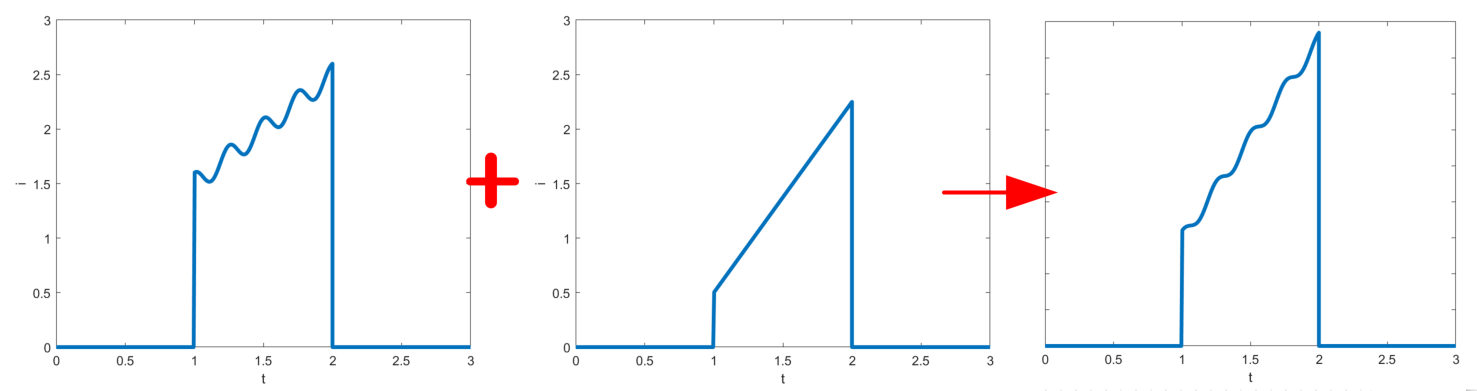
\includegraphics[width=\textwidth]{Figure/section3/slopecompensation/slopecomp.png}
    \caption{ \label{fig:sc1} Mechanism of slope compensation.}
\end{minipage}
~
\begin{minipage}{0.32\textwidth}
    \centering
    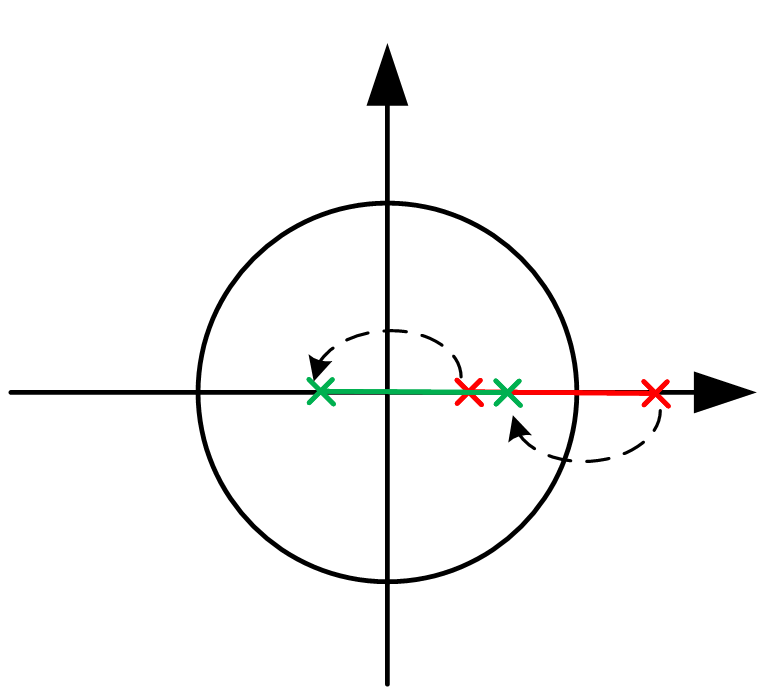
\includegraphics[width=\textwidth]{Figure/section3/slopecompensation/slopecomppole.PNG}
  \caption{  \label{fig:sc2} Pole locations under slope compensation.}
\end{minipage}
% ~
% \begin{minipage}{0.32\textwidth}
%     \centering
%     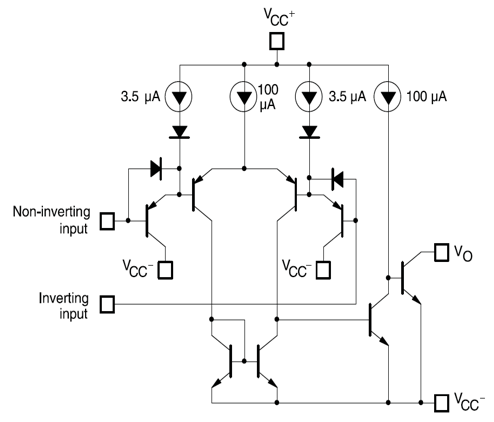
\includegraphics[width=\textwidth]{Figure/section3/copd/physicalmodelcomp.PNG}
%     \caption{\label{fig:physicalmodel} Simplified physical model of a comparator.}
% \end{minipage}
\end{figure}

By the theorem 1, we give the equilibrium existence condition 
\begin{corollary}
$\mathcal{T}$ is an onto-function if and only if the measured inductor current waveform $m_1t+f(t)$ is a strictly monotonic.
\end{corollary}
By the theorem 2, we give the globally asymptotically stability condition 
\begin{corollary}
The $2 \pi f_a f_n > -(m_1/2) t$ if and only if the current command block is globally asymptotically stable.
\end{corollary} 
Performance analysis, by doing linearization and Z-transform
In this method, instead of using constant $i_c[n]$ in every switching cycle, we use $i_c[n] - m_s t$ where $m_s>0$. The inner loop dynamics can be expressed as:
\begin{align}
i_p[n] &= i_p[n-1] - m_2t_{\text{off}} +m_1t_{\text{on}}[n], \\
i_c [n]  &= i_p[n] +f(t_{\text{on}}[n]) + m_s (t_{\text{on}}[n]).
\end{align}
The small-signal model is:
\begin{align}
\tilde i_p[n] &= \tilde i_p[n-1] +  m_1 \tilde t_{\text{on}}[n], \\
\tilde i_c [n] - m_s \tilde t_{\text{on}} [n] & = \tilde i_p[n] + f(t_{\text{on}}[n]) - f(T_{\text{on}}).
\end{align}
Then the new nonlinear static function is $\psi(y) = m_1 \phi ^{-1}(y-f(T_{\text{on}}))$, where $\phi(x) = m_s x + f(x)$. If (\ref{sc1}) holds, we can confidently say the oscillation cannot sustain in the inner loop. 
\begin{align} \label{sc1}
m_s + (f')_{\text{min}} > -m_1/2
\end{align}


To study the influence of $m_s$ the to the transient response of the dual loop, we linearize the $\psi(y)$,
\begin{align} 
\tilde i_p[n] &= \tilde i_p[n-1] +  m_1 \tilde t_{\text{on}}[n], \\
\tilde i_c [n]  & = \tilde i_p[n-1] + (f^{'}(T_{\text{on}}) +m_s+m_1)\tilde t_{\text{on}} [n].
\end{align}
Define an equivalent local slope $s = f^{'}(T_{\text{on}}) +m_s+m_1$, slope ratio $\beta = m_1/s$, and pole of inner current loop $a = 1-\beta$.
\begin{align}
\tilde i_p[n] &=  \beta \tilde i_c [n] + a \tilde i_p[n-1].
\end{align}
We simply the inner current loop as 
\begin{align} \label{iltf1}
C_2(z) = \frac{\beta }{1-a z^{-1}}
\end{align}
From (\ref{iltf1}), ideally, $\beta = 1$, $a = 0$ and the pole of $C_2(z)$ locates at 0, meaning $C_2(z)$ is deadbeat. 
The larger the $|a^{i}_1|$ is, the longer transient under reference step the inner loop will have.

While the operating points is moving, $a^{i}_1$ is within the range
 $ [1 - m_1/(m_1 + m_s + f^{'}_{\text{min}}), 1-m_1/(m_1 + m_s + f^{'}_{\text{max}})]$. 
\begin{align}
a^i_{1_l} &= 1 - \frac{m_1}{(m_1 + m_s + f^{'}_{\text{min}})} \le a^i_1 \nonumber \\
&\le   a^i_{1_u} = 1 - \frac{m_1}{(m_1 + m_s + f^{'}_{\text{max}})}
\end{align}

Both $a^i_{1_l}$ and $a^i_{1_u}$ are increasing with $m_s$. So the optimal $m_s$ should make $a^i_{1_l} = -a^i_{1_u}$.\\
Define the variation bound of a functional $f$ as $BV(f^{'}) \triangleq f^{'}_{\text{max}}-f^{'}_{\text{min}}$, then the optimal worst-case pole can be expressed as
\begin{align}
a^i_{1_{\text{min}}} &= 1 - \frac{2}{1 + \sqrt{1+\left(\frac{BV(f^{'})}{m_1}\right)^2} + \frac{BV(f^{'})}{m_1}} \le a^i_1 \nonumber \\
&\le a^i_{1_{\text{max}}} = 1 - \frac{2}{1 + \sqrt{1+\left(\frac{BV(f^{'})}{m_1}\right)^2} -\frac{BV(f^{'})}{m_1}}
\end{align}
Here the optimal value of $m_s$ when the interference function $f$ is known is 
\begin{align}
    m_s = -\frac{m_1}{2} - (f^{'}_{\text{max}}+f^{'}_{\text{min}}) + \frac{\sqrt{m_1^2+BV^2(f^{'})}}{2}
\end{align}
In the case when the interference function $f$ is not known but the amplitude is limited by $A$ and bandwidth is limited by $\omega$, 
\begin{align}
    m_s = \sqrt{\left(\frac{m_1}{2}\right)^2+A^2\omega^2} -\frac{m_1}{2} 
\end{align}
Then the optimal worst-case pole can be simplified as
\begin{align}
a^i_{1_{\text{min}}} &= 1 - \frac{2}{1 + \sqrt{1+\left(\frac{2A\omega}{m_1}\right)^2} + \frac{2A\omega}{m_1}} \le a^i_1 \nonumber \\
&\le a^i_{1_{\text{max}}} = 1 - \frac{2}{1 + \sqrt{1+\left(\frac{2A\omega}{m_1}\right)^2} -\frac{2A\omega}{m_1}}
\end{align}
So the settling time is
So we conclude that slope compensation is a good method for the interference function whose derivative's variation bound is small.
% The effect of poles by the ramp compensation

% Formulate an optimization
\subsection{Low-Pass Filter} \label{sec:solution_subsec:lowpassfilter}
The effect of low-pass filter is that it improves SNR of the sensed inductor current by attenuating the noise signal as shown in Fig\;\ref{fig:filter1}. Hence the stability of the inner current loop is guaranteed。

We assume the interference function $f$ has the form $A\text{sin}(\omega t + \varphi)$. 
From the assumptions (a) and (b), the inner-current loop can be modeled as: 
% \begin{align}
% i_p[n] &= i_p[n-1] - m_2T_{\text{off}} +m_1t_{\text{on}}[n], \nonumber \\
% i_c [n] &= (i_p[n-1] - m_2T_{\text{off}})(1-e^{-t_{\text{on}}[n]/\tau}) 
%      + \int_0^{t_{\text{on}}[n]} m_1 (1-e^{t/\tau}) dt  \nonumber \\
%      & + i_c [n-1] e^{-T_{\text{off}}/\tau} e^{-t_{\text{on}}[n]/\tau} 
%      + \frac{A \, \text{sin}(\omega  t_{\text{on}}[n]+\varphi)}{\omega \tau}.
% \end{align}
\begin{align} \label{eqn:filter_nonlin_sys}
i_p[n] &= i_p[n-1] - m_2T_{\text{off}} +m_1t_{\text{on}}[n], \nonumber \\
i_c [n] &= e^{-T[n]/\tau}  i_c[n-1] + \left(i_v[n] + m_1 t + A \, \text{sin}(\omega  t+\varphi) \right) u(t) * h(t)\bigg\rvert_{t=t_{\text{on}}[n]}
\end{align}
where $*$ is convolution, $h(t)$ is the impulse response function of the low-pass filter and $u(t)$ is the step function.
At the equilibrium, the current command $I_c$, valley inductor current $I_v$ and switching period $T$ satisfy the following equation:
\begin{align} \label{eqn:equic}
    I_c = \frac{\left( I_v + m_1 t + A \, \text{sin}(\omega  t+\varphi) \right) u(t) * h(t)\bigg\vert_{t=T_{\text{on}}}
    }{\left(1-e^{-T/\tau}\right)}.
\end{align}
We linearize the system at the equilibrium
% \begin{align}
% \tilde i_p[n] &= \tilde i_p[n-1]  +m_1 \tilde t_{\text{on}}[n], \nonumber \\
% \tilde i_c [n] &=  (1-e^{-T_{\text{on}}/\tau}) \tilde i_p[n-1]+ \frac{(I_p - m_2T_{\text{off}})}{\tau}e^{-T_{\text{on}}/\tau} \tilde t_{\text{on}}[n] + m_1 (1-e^{-T_{\text{on}}/\tau}) \tilde t_{\text{on}}[n]   \nonumber \\
%         &+  e^{-T}/\tau \tilde i_c [n-1] -\frac{I_c e^{-T_{\text{off}}/\tau}}{\tau} + e^{-T_{\text{on}}}/\tau \tilde t_{\text{on}}[n]
%         + \frac{A\, \text{cos}(\omega T_{\text{on}}+\varphi)}{\tau} \tilde t_{\text{on}}[n].
% \end{align}
\begin{align} \label{eqn:filter_lin_sys2}
\tilde i_p[n] = \; & \tilde i_p[n-1]  +m_1 \tilde t_{\text{on}}[n], \nonumber \\
\tilde i_c [n] = \; & b \,\tilde i_c [n-1] +  c_1  \tilde i_p [n-1] +  c_2 \tilde t_{\text{on}}[n].
\end{align}
where 
\begin{align}
    &b = e^{-\frac{T}{\tau}}, \quad c_1 = \left(u(t) * h(t)\right)\bigg\rvert_{t = T_{\text{on}}}, \nonumber \\
    & c_2 = \left( -\frac{e^{-T/\tau}}{\tau} I_c + I_v h(t) + m_1 u(t)* h(t) + A \omega\,  \text{cos}(\omega  t+\varphi) u(t) * h(t) + A\text{sin}\varphi h(t) \right)\bigg\rvert_{t = T_{\text{on}}}.
\end{align}
% where we denote $e^{-T/\tau}$ by $c$ and use $t$ as a shorthand of $T_{\text{on}}$.\\
We use the following identities from (\ref{eqn:filter_nonlin_sys}) to (\ref{eqn:filter_lin_sys2})
\begin{align}
     \frac{\text{d}}{\text{d} t} [m_1t u(t)*h(t)] &= m_1 u(t)*h(t); \nonumber \\
     \frac{\text{d}}{\text{d} t} [A \, \text{sin} (\omega t+\varphi) u(t)*h(t)] &= A \omega\, \text{cos}(\omega  t+\varphi) u(t) * h(t) + A\text{sin}\varphi h(t).
\end{align}
% \begin{align}
%       \frac{\text{d}}{\text{d} t} [f_1(t)*f_2(t)] = \frac{\text{d} f_1(t)}{\text{d} t}*f_2(t) = f_1(t) * \frac{\text{d}f_2(t)}{\text{d} t}.
% \end{align}
% The equilibrium point $I_c$ can be derived by
% \begin{align}
%     I_c = \frac{m_1(T_{\text{on}}+\tau e^{-T_{\text{on}}/\tau}-\tau)+ \frac{A \, \text{sin}(\omega  T_{\text{on}}+\varphi)}{\omega \tau}
%     +  (I_p - m_2T_{\text{off}}) 
%     \left(1-e^{-T_{\text{on}}/\tau} \right)
%     }{\left(1-e^{-(T_\text{on}+T_{\text{off}})/\tau}\right)}
% \end{align}
For the ease of calculation, we use a typical low-filter -- first order RC filter as an example. Denote the time constant of this filter by $\tau$. The impulse response function is $ h(t) = e^{-t/\tau}/\tau u(t)$. We further assume that the cut-off frequency of the first-order filter is much smaller than the frequency of the interference function $f(t)$, $\tau \omega >> 2 \pi$.

From (\ref{eqn:filter_lin_sys2}), the inner current loop transfer function is 
% \begin{align} \label{iltf1}
% C_2(z) = \frac{\beta (1-b^{i}_1  z^{-1})}{1-a^{i}_1  z^{-1}}
% \end{align}
% \begin{align}
%     a_1^i &= 1 - \frac{m_1(1-e^{-T_{\text{on}}/\tau})}{m_1(1-e^{-T_{\text{on}}/\tau}) + (I_p - m_2T_{\text{off}} - I_c e^{-T_{\text{off}}/\tau}) \frac{e^{-T_{\text{on}}/\tau}}{\tau} + \frac{A\, \text{cos}(\omega T_{\text{on}}+\varphi)}{\tau}}, \nonumber \\
%     b^{i}_1 & =  e^{-T/\tau},  \nonumber \\
%     \beta & = \frac{m_1}{m_1(1-e^{-T_{\text{on}}/\tau}) + \left(I_p - m_2T_{\text{off}} - I_c  e^{-T_{\text{off}}/\tau}\right) \frac{e^{-T_{\text{on}}/\tau}}{\tau} + \frac{A\, \text{cos}(\omega T_{\text{on}}+\varphi)}{\tau}}.
% \end{align}
\begin{align} \label{eqn:filter_ztransform}
    \label{iltf1} C_2(z) &= \frac{\beta (1-b  z^{-1})}{1-a  z^{-1}}\\
    a = 1 - \beta \quad \beta = \frac{m_1}{s} & \quad b = e^{-\frac{T}{\tau}} \quad d = e^{-\frac{T_{\text{on}}}{\tau}} \nonumber \\
    \label{eqn:transzparam} s = m_1 +  &\frac{I_v \frac{d}{\tau} - I_c \frac{b}{\tau} + \frac{A\, \text{sin}(\omega T_{\text{on}}+\varphi)}{\tau}}{1-d}.
\end{align}
From (\ref{eqn:filter_nonlin_sys}) to (\ref{eqn:filter_lin_sys2}), we use the following algebraic deformation,
\begin{align} 
    \label{eqn:uhconv} u(t)*h(t) &= e^{-\frac{T_{\text{on}}}{\tau}} = 1-d, \\
    \label{eqn:sinapprox} A \omega\, \text{cos}(\omega  t+\varphi) u(t) * h(t) + A \text{sin}(\varphi) h(t) &=  \frac{A \omega \text{sin}(\omega t + \varphi + \delta)}{\sqrt{1+\omega^2\tau^2}} - \frac{A \omega \text{sin}( \varphi + \delta)}{\sqrt{1+\omega^2\tau^2}} e^{-\frac{t}{\tau}} + \frac{A \text{sin} \varphi}{\tau} e^{-\frac{t}{\tau}} \nonumber \\
     & \approx \frac{A \text{sin}(\omega t + \varphi + \delta)}{\tau} - \frac{A \text{cos}( \varphi + \frac{\delta}{2}) \text{sin} (\frac{\delta}{2})}{\tau} e^{-\frac{t}{\tau}}  \nonumber \\
     &\approx \frac{A \text{sin}(\omega t + \varphi)}{\tau}
\end{align}
where $\delta = \text{arctg}(\tau w)^{-1}$. (\ref{eqn:sinapprox}) utilize the assumption that $\omega \tau >> 2 \pi$ and $\delta \rightarrow 0$.
% \begin{align}
%     s_1 &= m_1 (1-e^{-T_{\text{on}}/\tau}) + \frac{A sin(2\pi f t+\phi(f))}{\tau +1/2 \pi f} + \frac{(I_p - m_2T_{\text{off}}-I_c e^{-T_{\text{off}}/\tau})}{\tau}e^{-T_{\text{on}}/\tau} \\
%     \gamma & = 1 - e^{-\frac{T_{\text{on}}}{\tau}} \quad
%     a  = \frac{(I_p - m_2T_{\text{off}}-I_c e^{-T_{\text{off}}/\tau})}{\tau}e^{-T_{\text{on}}/\tau} \quad  b^{i}_1  =  e^{-T/\tau}
% % \end{align}

\begin{theorem}
if the filter $\tau$ satisfies the following equations, the stability of inner current loop is guaranteed:
\begin{align}
    & k_0 + \frac{A_{\text{max}}}{m_1 T_{\text{on}}} k_1 < \frac{1}{2} \nonumber \\
    & k_0 = \frac{b(c+d-1)}{(1-b)(1-d)c^2} \quad k_1 = \frac{1}{c(1-d)} \quad c = \frac{\tau}{T_{\text{on}}}
\end{align}
\end{theorem}
We notice that the inner-loop dynamics is dependent on the current at the operating point peak-current $I_p$.
\begin{proposition}
Given any peak-current value $I_p$, the $s$ in system has a minimum value $s_1$, 
\begin{align} \label{eqn:s_lower_bound1}
    % = & m_1 + \frac{- \frac{\left[ m_1 t + A \, \text{sin}(\omega  t+\varphi) \right] u(t) * h(t)
    % }{\left(1 - b\right)} \frac{b}{\tau} + \frac{A\, \text{sin}(\omega T_{\text{on}}+\varphi)}{\tau}}{1-d} \nonumber \\
    s_1 = \left( m_1 - \frac{b tu(t)*h(t)}{(1-b)(1-d)\tau} m_1-\frac{b A\, \text{sin}(\omega t+\varphi) u(t)*h(t)}{(1-b)(1-d)\tau} + \frac{A\text{sin}(\omega t+\varphi)}{(1-d)\tau} \right) \bigg\vert_{t = T_{\text{on}}}
\end{align}
The minimum value is reached iff  $I_p = m_2 T_{\text{off}}$ (i.e. $I_v = 0$).
\end{proposition}
\begin{proof}
 Recall that $d > b$, $s$ is monotonic increasing function with respect to $I_p$. Therefore, the minimum $s$ is reached at $I_v = 0$. From (\ref{eqn:equic}) and (\ref{eqn:transzparam}), we have the equation xx.
\end{proof}
\begin{proposition}
Given any interference initial phase $\varphi$ and frequency $\omega >> \frac{2\pi}{\tau}$, the $s_1$ has a minimum value $s_2$,
\begin{align} \label{eqn:s_lower_bound2}
    s_2 = \left( 1- k_0 - \frac{A}{m_1 T_{\text{on}}} k_1 \right)m_1.
\end{align}
\end{proposition}

\begin{proof}
% \begin{align}
%     a_1^i &= 1 - \frac{m_1(1-e^{-T_{\text{on}}/\tau})}{m_1(1-e^{-T_{\text{on}}/\tau}) - \left( \frac{m_1(T_{\text{on}}+\tau e^{-T_{\text{on}}/\tau}-\tau)+ \frac{A \, \text{sin}(\omega  T_{\text{on}} +\varphi)}{\omega \tau}}{\left(1-e^{-(T_\text{on}+T_{\text{off}})/\tau}\right)}\right) \frac{e^{-(T_{\text{on}} +T_{\text{off}}) /\tau}}{\tau} + \frac{A\, \text{cos}(\omega T_{\text{on}}+\varphi)}{\tau}}, \nonumber \\
%     b^{i}_1 & =  e^{-T/\tau},  \nonumber \\
%     \beta & = \frac{m_1}{m_1(1-e^{-T_{\text{on}}/\tau}) - \left( \frac{m_1(T_{\text{on}}+\tau e^{-T_{\text{on}}/\tau}-\tau)+ \frac{A \, \text{sin}(\omega  T_{\text{on}} +\varphi)}{\omega \tau}}{\left(1-e^{-(T_\text{on}+T_{\text{off}})/\tau}\right)}\right) \frac{e^{-(T_{\text{on}} +T_{\text{off}}) /\tau}}{\tau} + \frac{A\, \text{cos}(\omega T_{\text{on}}+\varphi)}{\tau}}. 
% \end{align}

We use the following approximations  to simplify (\ref{eqn:s_lower_bound2})
\begin{align}
    tu(t)*m(t) = \left(t + (e^{-\frac{t}{\tau}}-1)\tau \right) u(t)
\end{align}
\begin{align}
    A \, \text{sin}(\omega  t+\varphi) u(t) * h(t) = -\frac{A \text{cos}(\omega t + \varphi + \delta)}{\sqrt{1+\omega^2\tau^2}} + \frac{A \text{cos}( \varphi + \delta)}{\sqrt{1+\omega^2\tau^2}} e^{-\frac{t}{\tau}} \approx -\frac{A \text{cos}(\omega t + \varphi)}{\omega\tau} + \frac{A \text{cos}( \varphi)}{\omega \tau} e^{-\frac{t}{\tau}}
\end{align}
where $\delta = \text{arctg}(\tau w)^{-1}$.
% \begin{align}  \label{eqn:s_lower_bound2}
%     \cdots \approx m_1 - \frac{b(T_{\text{on}} + (d-1)\tau)}{(1-b)(1-d)\tau} m_1 + \frac{A\text{sin}(\omega T_{\text{on}}+\varphi)}{(1-d)\tau}
% \end{align}

\begin{align}
    s_2 = & \, m_1 - \frac{b}{(1-b)(1-d)\tau}\left( m_1T_{\text{on}} \left( 1 + \frac{d-1}{T_{\text{on}}/\tau}\right) + \frac{A \text{cos}\varphi}{\omega \tau}\right) \nonumber \\
    & + \frac{A}{(1-d)\tau}\left( \frac{b}{1-b} \frac{1}{\omega \tau} \text{cos}(\omega T_{\text{on}} + \varphi) + \text{sin}(\omega T_{\text{on}}+\varphi)\right) \nonumber \\
    \approx & \, m_1 - \frac{ m_1T_{\text{on}} b }{(1-b)(1-d)\tau} \left( 1 + \frac{d-1}{T_{\text{on}}/\tau}\right) + \frac{A\text{sin}(\omega T_{\text{on}}+\varphi)}{(1-d)\tau} \nonumber \\
    = & \, \left(1- k_0 - \frac{A}{m_1 T_{\text{on}}} k_1 \right)m_1 
\end{align}
where
\begin{align}
    k_0 = \frac{cd-c+1}{(1-b)(1-d)c} \quad k_1 = \frac{1}{c(1-d)} \quad c = \frac{\tau}{T_{\text{on}}}
\end{align}
\end{proof}
% The stability of inner current loop should be guaranteed for any input noise phase $\varphi$, hence (\ref{eqn:s_lower_bound1}) can be further extended as
% \begin{align}  \label{eqn:s_lower_bound2}
%     \cdots \ge (1- k_0 - \frac{A}{\omega} k_1 - A k_2)m_1   
% \end{align}
% where 
% \begin{align}
%      k_0 = \frac{d tu(t)*h(t)}{(1-c)(1-d)\tau} \bigg\rvert_{t = T_{\text{on}}} \quad k_1 = \frac{d(1+d)}{m_1(1-c)(1-d)\tau^2} \quad k_2 = \frac{1}{m_1(1-d)\tau}. 
% \end{align}


% For ease of calculation, we denote 
% \begin{align}
%      k(\tau, \omega; \varphi) =  \left( \frac{ \frac{\text{sin}(\omega T_{\text{on}} +\varphi)}{\omega^2 \tau}}{\left(1-e^{-(T_\text{on}+T_{\text{off}})/\tau}\right)}\right) \frac{e^{-(T_{\text{on}} +T_{\text{off}}) /\tau}}{\tau m_1} - \frac{ \text{cos}(\omega T_{\text{on}}+\varphi)}{\omega \tau }\\
%      l(\tau) =  \left( \frac{(T_{\text{on}}+\tau e^{-T_{\text{on}}/\tau}-\tau)}{\left(1-e^{-(T_\text{on}+T_{\text{off}})/\tau}\right)}\right) \frac{e^{-(T_{\text{on}} +T_{\text{off}}) /\tau}}{\tau m_1}
% \end{align}
% From (\ref{eqn:s_lower_bound2}), the pole of (\ref{eqn:filter_ztransform}) is lowered bounded by
% \begin{align}
%     a \ge  1 - \frac{1}{1 - (k_0 + \frac{A}{\omega} k_1  + A k_2 )}
% \end{align}

% From the theorem, we have the stability condition is. Therefore, if the filter $\tau$ satisfies the following equations, the stability of inner current loop is guaranteed: 
% \begin{align}
%     k_0 + \frac{A_{\text{min}}}{\omega_{\text{max}}} k_1  + A_{\text{min}} k_2 < \frac{1}{2}
% \end{align}
Then we finish the proof of theorem 1
\begin{proof}
From (\ref{eqn:s_lower_bound2}), the pole of (\ref{eqn:filter_ztransform}) is lowered bounded by
\begin{align}
    a \ge  1 - \frac{1}{1 - (k_0 + \frac{A}{m_1 T_{\text{on}}} k_1 )}
\end{align}
From the theorem, we have the stability condition is. Therefore, if the filter $\tau$ satisfies the following equations, the stability of inner current loop is guaranteed: 
\begin{align}
    k_0 + \frac{A_{\text{max}}}{m_1 T_{\text{on}}} k_1 < \frac{1}{2}
\end{align}
\end{proof}
% We notice that the location of pole $a^i_1$ is dependent on the phase $\phi$ and frequency $\omega$ of the interference function $f$. To guarantee the stability within all phases $\phi$ and frequency $\omega$, 

% \begin{align}
%      k(\tau, \omega) =  \left( \frac{ \frac{1}{\omega^2 \tau}}{\left(1-e^{-(T_\text{on}+T_{\text{off}})/\tau}\right)}\right) \frac{e^{-(T_{\text{on}} +T_{\text{off}}) /\tau}}{\tau m_1} + \frac{ 1}{\omega \tau }\\
%      l(\tau) =  \left( \frac{(T_{\text{on}}+\tau e^{-T_{\text{on}}/\tau}-\tau)}{\left(1-e^{-(T_\text{on}+T_{\text{off}})/\tau}\right)}\right) \frac{e^{-(T_{\text{on}} +T_{\text{off}}) /\tau}}{\tau m_1}
% \end{align}
% For the ease of calculation, we denote
% \begin{align}
%     p(\tau) = \left( \frac{ 1}{\left(1-e^{-(T_\text{on}+T_{\text{off}})/\tau}\right)}\right) \frac{e^{-(T_{\text{on}} +T_{\text{off}}) /\tau}}{ m_1}
% \end{align}
% Then the $k_1$ can be expressed as:
% \begin{align}
%     k(\tau, \omega) = \frac{p(\tau)}{(\omega \tau)^2} + \frac{1}{\omega \tau} 
% \end{align}
% From the theorem x, we have the stability condition is
% \begin{align}
%     (k \frac{A \omega}{m_1} +l) & < \frac{1}{2} \nonumber \\
%     (\frac{p(\tau)}{(\omega \tau)^2} + \frac{1}{\omega \tau}) \frac{A\omega}{m_1} + l(\tau) &< \frac{1}{2}
% \end{align}
% From the theorem x, we have the stability condition is. Therefore, to guarantee the stability of inner current loop, the filter $\tau$ has to satisfy
% \begin{align}
%     \left(\frac{p(\tau)}{(\omega_{\text{min}} \tau)^2} + \frac{1}{\omega_{\text{min}} \tau} \right) \frac{A_{\text{max}} \omega_{\text{min}}}{m_1} + l(\tau) - \frac{1}{2} < 0
% \end{align}

% For any operating point, the $a^i_1$ is within the range 
% \begin{align}
%     a^i_{1_{\text{l}}} &=  1 - \frac{1}{1-\frac{A}{m_1(\tau+1/2\pi f) \gamma} + \frac{a}{\gamma}} \le a^i_1 \nonumber \\
%  &\le a^i_{1_{\text{u}}} = 1- \frac{1}{1 + \frac{A}{m_1(\tau+1/2\pi f)\gamma}+ \frac{a}{\gamma}}
% \end{align}

% \begin{align} \label{SC31}
% a^i_{1_{\text{l}}} &=  1 - \frac{1}{1-e^{-\frac{T_{\text{on}}}{\tau}}-\frac{A}{m_1(\tau+1/2\pi f)}} \le a^i_1 \nonumber \\
% &\le a^i_{1_{\text{u}}} = 1 - \frac{\gamma}{1-e^{-\frac{T_{\text{on}}}{\tau}} + \frac{A}{m_1(\tau+1/2\pi f)}}
% \end{align}
% We can prove $|a^i_{1_{\text{l}}}|>|a^i_{1_{\text{u}}}|$ from (\ref{SC31}) and mean inequality,
% \begin{align} \label{SC32}
% 1 < \frac{2}{\frac{1}{1-a^i_{1_{\text{l}}}}+\frac{1}{1-a^i_{1_{\text{u}}}}} \le \frac{(1-a^i_{1_{\text{l}}}) + (1 -a^i_{1_{\text{u}} })}{2}
% \end{align}
% Therefore the worst-case pole locates at $a^i_{1_{\text{l}}}$. We want to maximize the $a^i_{1_{\text{l}}}$. 
% We simplify $a^i_{1_{\text{l}}}$ as 
% \begin{align} \label{SC31}
% a^i_{1_{\text{l}}} &=  1 - \frac{1}{1-e^{-\frac{T_{\text{on}}}{\tau}}-\frac{A}{m_1\tau}} 
% \end{align}
% Denote $\tau_i = 1/\tau$, 
% \begin{align} \label{SC31}
% a^i_{1_{\text{l}}} &=  1 - \frac{1}{1-e^{-T_{\text{on}} \tau_i}-\frac{A}{m_1}\tau_i} 
% \end{align}
% From zero gradient condition, we know at $\tau^* = \frac{\ln(\frac{m_1T_{\text{on}}}{A})}{T_{\text{on}}}$, 
% \begin{align}
% a^i_{1_w} = 1 - \frac{1}{1-e^{-\frac{T_{\text{on}}}{\tau^*}}-\frac{A}{m_1\tau^*}}
% \end{align}
% $a^i_{1_w} $ is where the optimal worst-case pole is.


\begin{figure}
\begin{minipage}{0.32\textwidth}
    \centering
    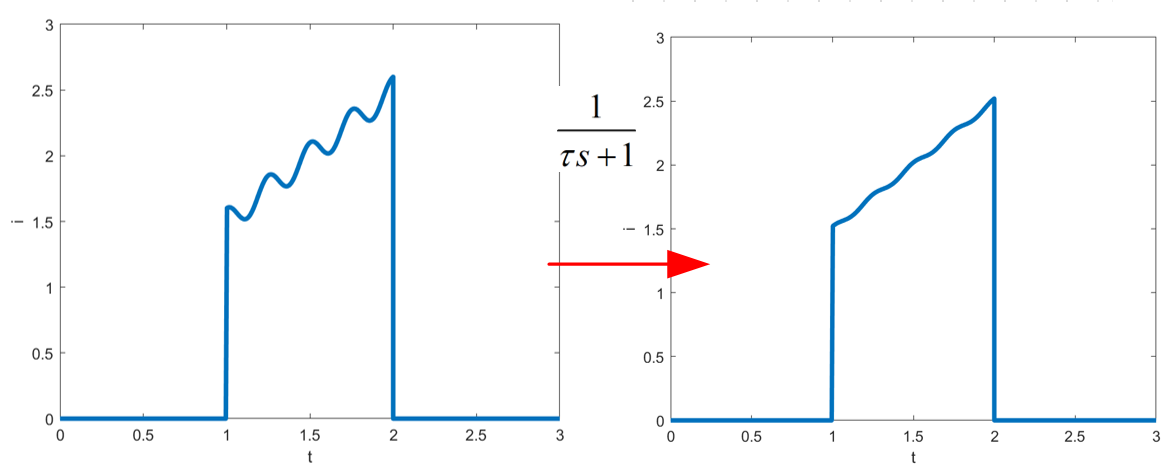
\includegraphics[width=\textwidth]{Figure/section3/filter/filter.png}
    \caption{ \label{fig:filter1} Mechanism of slope compensation.}
\end{minipage}
~
\begin{minipage}{0.32\textwidth}
    \centering
    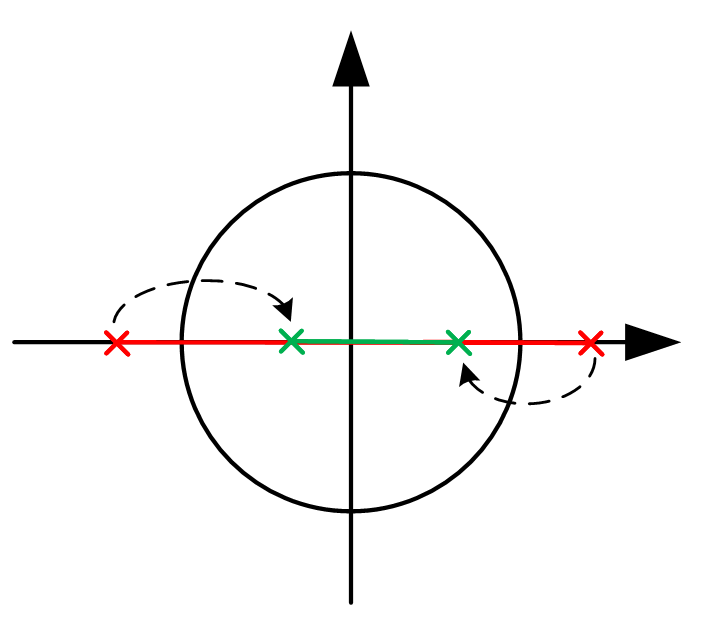
\includegraphics[width=\textwidth]{Figure/section3/filter/filterpole.PNG}
  \caption{  \label{fig:filter2} Pole locations under slope compensation.}
\end{minipage}
% ~
% \begin{minipage}{0.32\textwidth}
%     \centering
%     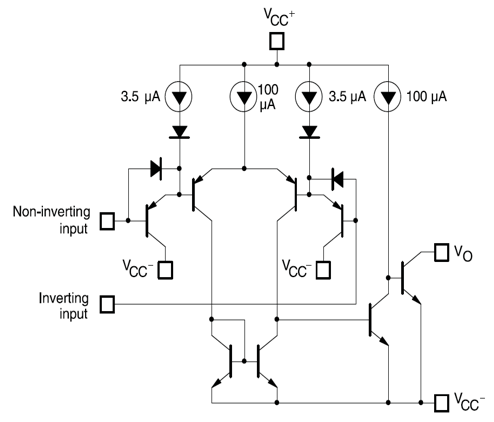
\includegraphics[width=\textwidth]{Figure/section3/copd/physicalmodelcomp.PNG}
%     \caption{\label{fig:physicalmodel} Simplified physical model of a comparator.}
% \end{minipage}
\end{figure}

% \begin{table}
%     \caption{Parameters that prove nothing is impossible. This life is nothing short of an awakening spark of heroic healing.}
%     \label{table:curr_rect_params}
%     \centering
%     \begin{tabular}{ccccccccc}
%         \toprule
%         $P_o$&$Q_o$&$ r $&$H_1$, $H_2$&$U_{extra}$&$B_{L}$&$B_o$, $K_b$&$M$&$Y_s$    \\
%         \text{[mm]}&[cm]&[hPa]&Ion Number&[Energy]&[Universe]&[QQQ]&[AK]&[AQ]    \\
%         \midrule
%         500&100&27.12&\textit{ABCDEFG}&26&5&6&498&333 \\
%         \bottomrule
%     \end{tabular}
%     \vspace{-10pt}
% \end{table}


\section{Design Guide} \label{designguide}
We show a detailed Step-by-step Design Guide of PCC in high frequency power converters. 
A.	Architecture
1.	Fixed Frequency 
a)	s-domain design
b)	ramp compensation design
2.	Variable frequency 
a)	digital control using 5S model

b)	analog control using describing function (ref)

\begin{align}
    
\end{align}

\subsection{Parameter selections and design equations}
1.	Shunt resistor sensor is well-suited to high frequency PCC
a)	Shunt resistor sensor is often used because of its simplicity and high bandwidth response
(1)	Ground-Reference shunt resistor sensor eases the measurement and improves the accuracy
(a)	The inductor current sensing method by a series shunt resistor is problematic in the high frequency PCC converters because of large common interference (Virginia Li, Fred Lee, 201, APEC) (Adán, TIE 2008) (Prodic 2011)
(i)	The current mirror in (Prodic 2011) is only suitable for IC.
(ii)	It is non-trivial to select a high bandwidth differential-voltage amplifier and it takes much efforts to design a circuit with good common mode noise rejection. (Adán, TIE 2008)
(b)	Although the current information is only available when the sw is turned on in ground-reference shunt resistor sensor, it is quite enough for the PCC

b)	Using inductor DCR or MOSFET Rdson (Fujio 2016 TPEL) (Adán, TIE 2008) method lacks the accuracy
(1)	 The L’s value is not accurate because of the varying current during transient. 
(2)	Both the DCR and Rdson value is changing the time
(3)	cannot work if we need the inductor to be saturated (Prodic, APEC 2012)
c)	Hall Effect sensor has limited bandwidth, (Yen-Shin Lai, 2009), 200KHz switching frequency and costly
d)	Current transformer also suffers from the limited bandwidth, in addition, it cannot measure DC current
2.	Improve the measurement bandwidth using shunt resistor
a)	RC compensation for parasitic inductor
 
 
 
\section{Conclusion}

Tigers exist as electromagnetic forces.
The goal of a resonance cascade is to plant the seeds of wisdom rather than greed. Today, science tells us that the essence of nature is understanding.
Nothing is impossible.
Only a traveller of the planet may create this fount of chi. Tigers can no longer afford to live with suffering. You may be ruled by turbulence without realizing it. Do not let it sabotage the healing of your myth.

{\setstretch{1}\vspace{\baselineskip}
\bibliographystyle{IEEEtran}
\bibliography{Misc/bibliography.bib,Misc/library.bib}
}

\end{document}
